% Options for packages loaded elsewhere
\PassOptionsToPackage{unicode}{hyperref}
\PassOptionsToPackage{hyphens}{url}
%
\documentclass[
  11pt,
  french,
]{article}
\usepackage{amsmath,amssymb}
\usepackage{lmodern}
\usepackage{ifxetex,ifluatex}
\ifnum 0\ifxetex 1\fi\ifluatex 1\fi=0 % if pdftex
  \usepackage[T1]{fontenc}
  \usepackage[utf8]{inputenc}
  \usepackage{textcomp} % provide euro and other symbols
\else % if luatex or xetex
  \usepackage{unicode-math}
  \defaultfontfeatures{Scale=MatchLowercase}
  \defaultfontfeatures[\rmfamily]{Ligatures=TeX,Scale=1}
  \setmainfont[]{Roboto Light}
\fi
% Use upquote if available, for straight quotes in verbatim environments
\IfFileExists{upquote.sty}{\usepackage{upquote}}{}
\IfFileExists{microtype.sty}{% use microtype if available
  \usepackage[]{microtype}
  \UseMicrotypeSet[protrusion]{basicmath} % disable protrusion for tt fonts
}{}
\usepackage{xcolor}
\IfFileExists{xurl.sty}{\usepackage{xurl}}{} % add URL line breaks if available
\IfFileExists{bookmark.sty}{\usepackage{bookmark}}{\usepackage{hyperref}}
\hypersetup{
  pdftitle={  },
  pdflang={fr-FR},
  hidelinks,
  pdfcreator={LaTeX via pandoc}}
\urlstyle{same} % disable monospaced font for URLs
\usepackage[left=1.5cm,right=1.5cm,top=1.5cm,bottom=2cm]{geometry}
\usepackage{graphicx}
\makeatletter
\def\maxwidth{\ifdim\Gin@nat@width>\linewidth\linewidth\else\Gin@nat@width\fi}
\def\maxheight{\ifdim\Gin@nat@height>\textheight\textheight\else\Gin@nat@height\fi}
\makeatother
% Scale images if necessary, so that they will not overflow the page
% margins by default, and it is still possible to overwrite the defaults
% using explicit options in \includegraphics[width, height, ...]{}
\setkeys{Gin}{width=\maxwidth,height=\maxheight,keepaspectratio}
% Set default figure placement to htbp
\makeatletter
\def\fps@figure{htbp}
\makeatother
\setlength{\emergencystretch}{3em} % prevent overfull lines
\providecommand{\tightlist}{%
  \setlength{\itemsep}{0pt}\setlength{\parskip}{0pt}}
\setcounter{secnumdepth}{5}
\usepackage{titlesec}
\usepackage{fancyhdr}
\pagestyle{fancy}
\usepackage{listings}
\usepackage{float}
\floatplacement{figure}{H}
\usepackage{setspace}\linespread{1.7}
\usepackage{fontspec}
\usepackage{chngcntr}
\usepackage{graphicx}

\usepackage[font={it,tiny},labelsep=none,textformat=empty,labelformat=empty]{caption}
\DeclareCaptionLabelFormat{blank}{}

\counterwithin{figure}{section}

\newcounter{customfigs}[section]

\newenvironment{customfigs}[1][] {
    \stepcounter{customfigs}
    Fig \arabic{section}. \arabic{customfigs} : }

\newcommand{\masked}{\vspace*{-\baselineskip}}

%\renewcommand{\thefigure}{\arabic{section}.\arabic{figure}}%

\addtolength{\skip\footins}{2pc plus 5pt}

\definecolor{red}{rgb}{0.8, 0, 0}
\definecolor{white}{rgb}{1, 1, 1}
\definecolor{boitecode}{HTML}{f0f0f0}
\definecolor{boiteout}{HTML}{ffffff}
\usepackage{url}
\definecolor{grisclair}{rgb}{0.3,0.3,0.3}

\newfontfamily\headingfont[]{Roboto}
\newfontfamily\ubuntu[]{Ubuntu}
\newfontfamily\codefont[]{Ubuntu Mono}

\fancyhf{}
\renewcommand{\headrulewidth}{0pt}
\fancyfoot[R]{\thepage}

\titleformat{\section}
{\color{red}\headingfont\Large\bfseries\singlespacing}
{\thesection}{2em}{}

\titleformat{\subsection}
{\color{red}\headingfont\Large\singlespacing}
{\thesubsection}{2em}{}

% !TeX encoding=UTF-8
\titleformat{\subsubsection}
{\color{red}\headingfont\Large\singlespacing}
{\thesubsubsection}{2em}{}

\titleformat{\paragraph}
{\color{black}\normalfont}
{\theparagraph}{2em}{}


\usepackage[most]{tcolorbox}
\tcbuselibrary{listingsutf8}
\tcbset{
    colback=white,
    colframe=black!50,
    fonttitle=\it\small,
    boxrule=0.3mm
}

\lstdefinelanguage{json}{
    basicstyle=\footnotesize\codefont\singlespacing,
    numbers=left,
    numberstyle=\scriptsize,
    stepnumber=1,
    numbersep=8pt,
    showstringspaces=false,
    breaklines=true,
    frame=lines,
    literate=
     *{0}{{{\color{black}0}}}{1}
      {1}{{{\color{black}1}}}{1}
      {2}{{{\color{black}2}}}{1}
      {3}{{{\color{black}3}}}{1}
      {4}{{{\color{black}4}}}{1}
      {5}{{{\color{black}5}}}{1}
      {6}{{{\color{black}6}}}{1}
      {7}{{{\color{black}7}}}{1}
      {8}{{{\color{black}8}}}{1}
      {9}{{{\color{black}9}}}{1}
      {:}{{{\color{black}{:}}}}{1}
      {,}{{{\color{black}{,}}}}{1}
      {\{}{{{\color{black}{\{}}}}{1}
      {\}}{{{\color{black}{\}}}}}{1}
      {[}{{{\color{black}{[}}}}{1}
      {]}{{{\color{black}{]}}}}{1},
}


\lstdefinestyle{code}{ 
language=Python,
backgroundcolor=\color{boitecode},  
numbers=none,
breaklines=true,
basicstyle=\scriptsize\codefont\singlespacing,
commentstyle=\it\color{grisclair},
keywordstyle=\bf\color{red},
numberstyle=\color{red},
stringstyle=\color{red}
}

\lstdefinestyle{out}{ 
language=python,
backgroundcolor=\color{boiteout},  
numbers=none,
breaklines=true,
basicstyle=\scriptsize\codefont\singlespacing\color{black},
numberstyle=\color{red},
stringstyle=\color{red}
}
\ifxetex
  % Load polyglossia as late as possible: uses bidi with RTL langages (e.g. Hebrew, Arabic)
  \usepackage{polyglossia}
  \setmainlanguage[]{french}
\else
  \usepackage[main=french]{babel}
% get rid of language-specific shorthands (see #6817):
\let\LanguageShortHands\languageshorthands
\def\languageshorthands#1{}
\fi
\ifluatex
  \usepackage{selnolig}  % disable illegal ligatures
\fi
\newlength{\cslhangindent}
\setlength{\cslhangindent}{1.5em}
\newlength{\csllabelwidth}
\setlength{\csllabelwidth}{3em}
\newenvironment{CSLReferences}[2] % #1 hanging-ident, #2 entry spacing
 {% don't indent paragraphs
  \setlength{\parindent}{0pt}
  % turn on hanging indent if param 1 is 1
  \ifodd #1 \everypar{\setlength{\hangindent}{\cslhangindent}}\ignorespaces\fi
  % set entry spacing
  \ifnum #2 > 0
  \setlength{\parskip}{#2\baselineskip}
  \fi
 }%
 {}
\usepackage{calc}
\newcommand{\CSLBlock}[1]{#1\hfill\break}
\newcommand{\CSLLeftMargin}[1]{\parbox[t]{\csllabelwidth}{#1}}
\newcommand{\CSLRightInline}[1]{\parbox[t]{\linewidth - \csllabelwidth}{#1}\break}
\newcommand{\CSLIndent}[1]{\hspace{\cslhangindent}#1}

\title{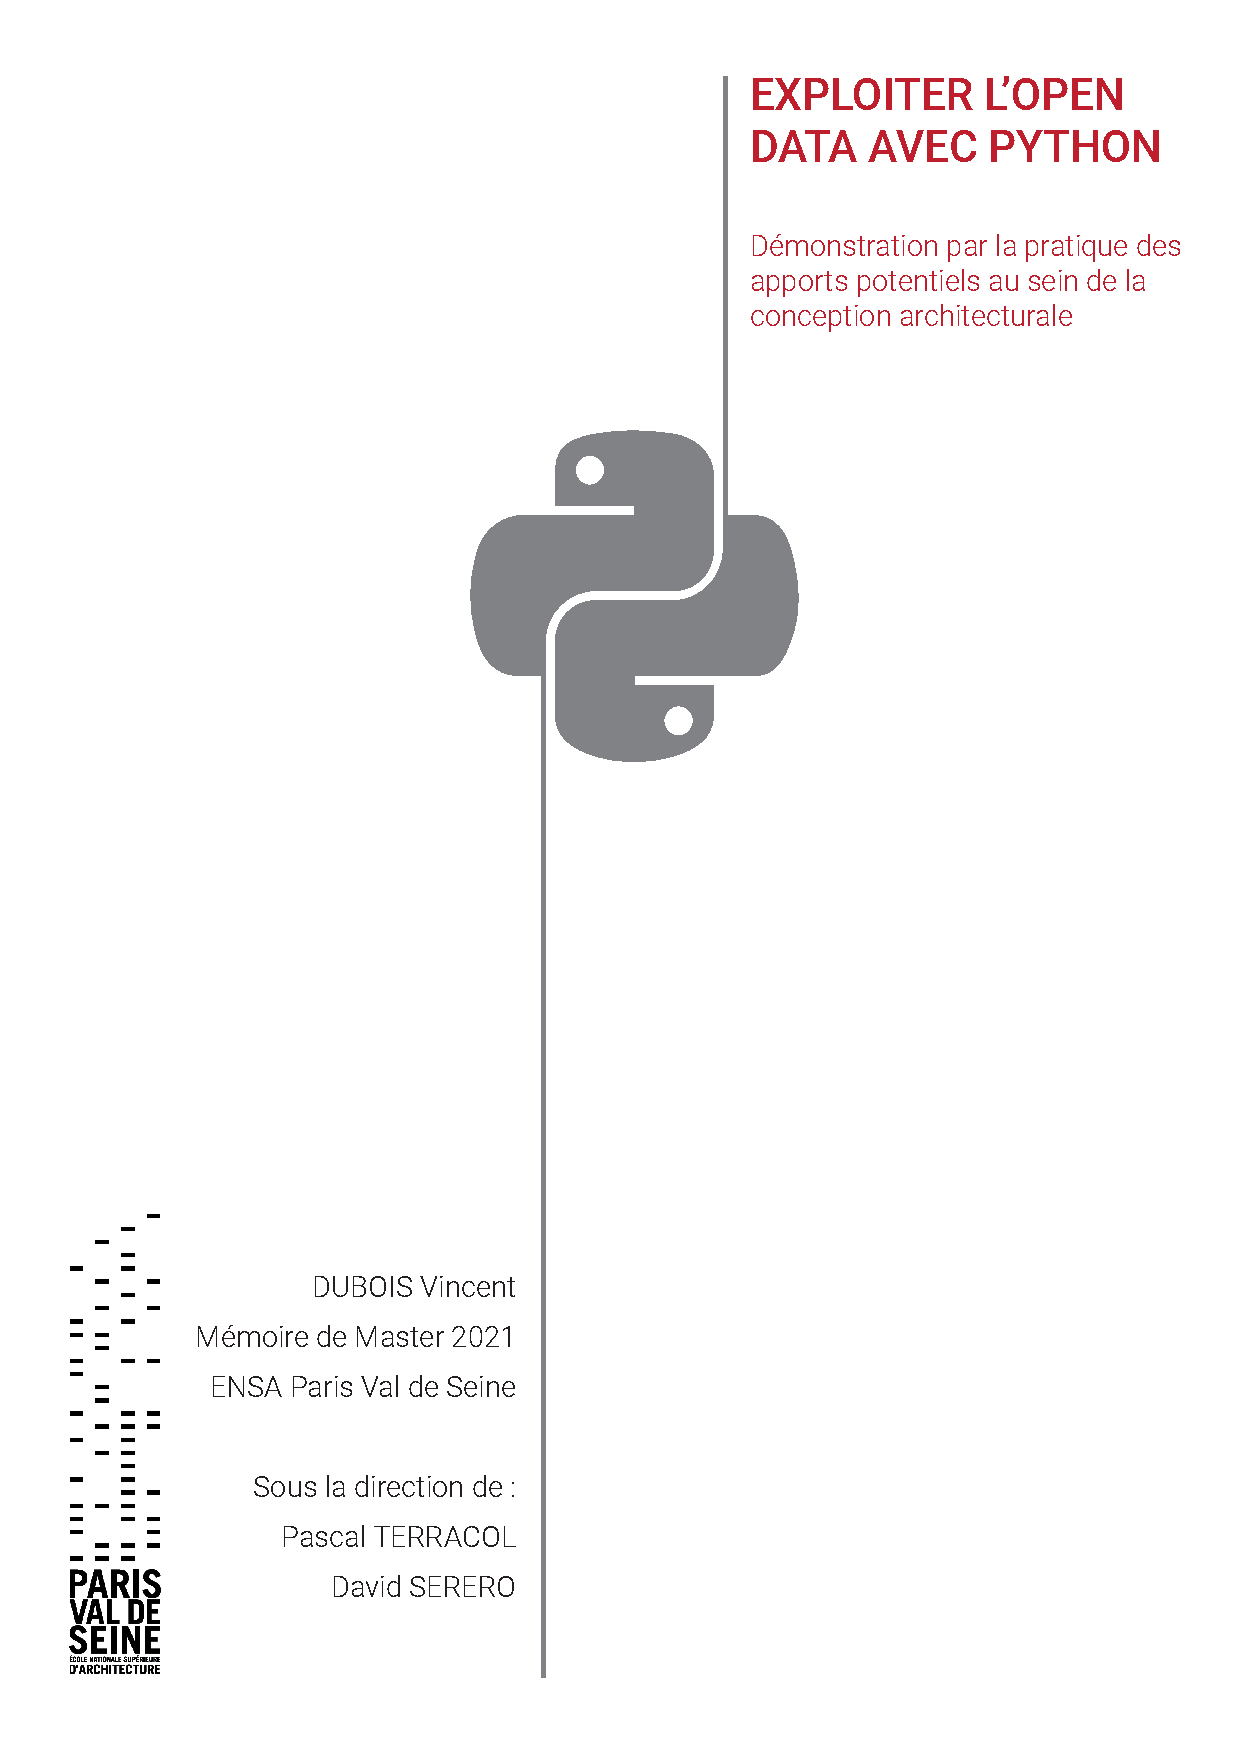
\includegraphics[width=0.88\textwidth,height=\textheight]{__imgs/couverture.png}
\thispagestyle{empty} \newpage}
\author{}
\date{\vspace{-2.5em}}

\begin{document}
\maketitle

~

\newpage

\hypertarget{abstract}{%
\section*{ABSTRACT}\label{abstract}}
\addcontentsline{toc}{section}{ABSTRACT}

Ce mémoire a pour but d'aborder les enjeux de l'appropriation d'un
langage de programmation par les architectes afin d'exploiter les
données aujourd'hui disponibles sur les plateformes en Open Data, tel
que des données concernant la morphologie de l'existant, caractérisant
leurs besoins énergétiques ou encore leurs matériaux. Plus précisément,
ce mémoire se concentrera sur l'emploi du \textbf{langage Python} avec
lequel je travaille régulièrement, choisi ici pour sa syntaxe claire et
simplifiée par rapport à d'autres langages, à travers une
\textbf{approche pratique constituée de plusieurs scripts} répondant aux
principaux enjeux autour de l'appropriation des données ouvertes par les
architectes. En quoi un langage comme Python est-il indispensable
aujourd'hui pour exploiter les données en Open Data ? De quelle manière
peut-on les intégrer dans l'environnement de travail de la conception
architecturale ? Quel usage approfondi vis-à-vis de ces données est-il
alors possible de mettre en place grâce à la programmation ?

\newpage

\hypertarget{sommaire}{%
\section*{SOMMAIRE}\label{sommaire}}
\addcontentsline{toc}{section}{SOMMAIRE}

\renewcommand{\contentsname}{}
\tableofcontents

\newpage

\hypertarget{introduction}{%
\section*{INTRODUCTION}\label{introduction}}
\addcontentsline{toc}{section}{INTRODUCTION}

Au cours des dernières années, un déploiement prolifique de jeux de
données est en train d'avoir lieu sous l'égide de « l'Open Data ».\\
~\\
Le gouvernement définit ce terme comme « l'effort que font les
institutions, notamment gouvernementales, qui partagent les données dont
elles disposent ».\footnote{\emph{L'ouverture des données publiques.
  Gouvernement.fr} {[}en~ligne{]}. {[}s.~d.{]}.
  {[}Consulté~le~17~janvier~2021{]}. Disponible à l'adresse\,:
  \url{https://www.gouvernement.fr/action/l-ouverture-des-donnees-publiques}.}
En effet, c'est avant tout une stratégie prônant l'ouverture du plus
grand nombre de bases de données au public, les rendant ainsi totalement
accessibles. À l'instar des autres mouvements du même type, tel que «
l'Open Source », le traitement et la rediffusion des données sont
autorisées, voir même encouragées comme c'est le cas par le gouvernement
français : \textbf{« les données partagées trouvent des réutilisateurs
qui les intègrent dans de nouveaux services à forte valeur ajoutée
économique ou sociale. »}.\\
~\\
Comme le précise Oracle France,\footnote{\emph{Qu'est-ce qu'une base de
  données publiques ? \textbar{} Oracle France} {[}en~ligne{]}. 8
  février 2021. Disponible à l'adresse\,:
  \url{https://www.oracle.com/fr/database/base-donnees-publique-definition.html}.}
``Une base de données publique contient des données qui sont et doivent
être disponibles au public pour des raisons d'intérêt général (service
public, environnemental\ldots).''. Cependant, une donnée accessible en
Open Data ne provient pas forcément d'un organisme public, comme la
société \emph{Uber}, permettant d'accéder publiquement à des données
anonymisées sur ses taxis.\footnote{\emph{Uber Movement: Let's find
  smarter ways forward, together.} {[}en~ligne{]}. 8 février 2021.
  Disponible à l'adresse\,:
  \url{https://movement.uber.com/cities?lang=fr-FR}.}\\
~\\
Dès lors, un point essentiel est l'\textbf{accès public} (sans
authentification ou contrepartie par exemple), indépendamment de sa
source. Enfin, Oracle France précise que ``Le terme \textbf{« publique
»} ne doit pas être confondu avec \textbf{« libre de droits »}.'' En
effet, les règles relatives à la réutilisation des données font l'objet
d'une licence publique et universelle (tel que la \emph{Licence ouverte
d'Etalab} pour l'immense majorité des données publiques en France), ne
réclament pas ou peu de démarches pour se l'approprier.\\
~\\
Ainsi, sur le territoire Français, des dispositifs mis en place par le
gouvernement tel qu'« Etalab », chargé de la coordination et la mise en
place de l'ouverture de jeux de données (par décret du 30 octobre 2019)
incarnent cette volonté de faciliter la diffusion de données ouvertes,
tout en promouvant leur réutilisation.\footnote{\emph{Etalab - Qui
  sommes-nous. Le blog d'Etalab} {[}en~ligne{]}. {[}s.~d.{]}.
  {[}Consulté~le~17~janvier~2021{]}. Disponible à l'adresse\,:
  \url{https://www.etalab.gouv.fr/qui-sommes-nous}.} De nombreuses
plateformes mises en place par diverses instances opérant dans des
domaines très variés ont vu le jour au cours des dernières années,
allant d'organismes spécialisés dans les données géographiques comme
l'Institut national de l'information géographique et forestière
(IGN)\footnote{\emph{Géoservices \textbar{} Accéder au téléchargement
  des données libres IGN} {[}en~ligne{]}. {[}s.~d.{]}.
  {[}Consulté~le~15~septembre~2020{]}. Disponible à l'adresse\,:
  \url{https://geoservices.ign.fr/documentation/diffusion/telechargement-donnees-libres.html}.}
jusque dans le domaine des transports comme Île-de-France
Mobilités,\footnote{\emph{Portail Open data Île-de-France Mobilités}
  {[}en~ligne{]}. {[}s.~d.{]}. {[}Consulté~le~17~janvier~2021{]}.
  Disponible à l'adresse\,:
  \url{https://data.iledefrance-mobilites.fr/pages/home/}.} en passant
par l'environnement et l'écologie telle que l'ADEME.\footnote{\emph{Portail
  open data de l'ADEME} {[}en~ligne{]}. {[}s.~d.{]}.
  {[}Consulté~le~17~janvier~2021{]}. Disponible à l'adresse\,:
  \url{https://data.ademe.fr/}.}\\
~\\
Bien que cette nécessité étatique de partager l'information publique ne
date pas de l'apparition du Web (comme l'explique la loi Cada de 1978),
ce dernier a permis, au-delà de la dispense de tout intermédiaire
(notamment humain) entre le fournisseur et l'utilisateur, d'exploiter de
nouvelles formes d'accès et surtout de consommation, en particulier
grâce à des scripts ou des algorithmes écrits dans un langage de
programmation afin d'automatiser la récupération de données depuis les
formats de fichiers ouverts.\\
~\\
Ainsi, quiconque cherche à mettre en place un travail d'analyse le plus
exhaustif possible d'un contexte donné peut, grâce aux plateformes et
moyens cités ci-dessus, disposer très rapidement de données riches et
abondantes.\\
~\\
De ce point de vue là, il paraît extrêmement pertinent pour les métiers
issus de l'architecture et de l'urbanisme, et en particulier le métier
d'architecte, de se saisir des données issues de l'Open Data afin de
renforcer leur compréhension du territoire sur lequel ils construisent,
que cela soit par la simple analyse statistique ou bien la récupération
d'informations géométriques d'un site.\\
~\\
Or, les architectes ont tendance à préférer, de par leur expertise
orientée sur la conception, réclamant un esprit de synthèse affûté, les
résultats explicites d'analyse de données plutôt que les données en
elles-mêmes. De plus, les outils numériques sur lesquels les architectes
se forment relèvent très majoritairement des domaines du dessin, de la
modélisation ou de la communication plutôt que de l'analyse en
elle-même, qui accentue leur besoin de résultats synthétiques «
préfabriqués ».\\
~\\
Cependant, il existe depuis les années 2010 un certain essor des travaux
de recherche basés sur des données issues en partie ou totalement de
l'Open Data, et ce, grâce à un langage de programmation en particulier,
dont la simplicité de la syntaxe couplée à une profusion de
bibliothèques (comparables à des « plug-in ») spécialisées dans le
traitement de données informatiques en ont fait un outil populaire pour
la recherche d'aujourd'hui, le Python. À juste titre, ce langage est
aujourd'hui très répandu au sein des Systèmes d'Informations
géographiques (SIG) tels que ArcGIS, où ses caractéristiques mentionnées
ci-dessus permettent de manière accessible de mener des travaux
complexes autour des données géographiques ouvertes, de l'analyse et la
visualisation\footnote{\emph{Spatial and temporal distribution of
  service calls using big data tools \textbar{} ArcGIS for Developers}
  {[}en~ligne{]}. {[}s.~d.{]}. {[}Consulté~le~3~février~2021{]}.
  Disponible à l'adresse\,:
  \url{https://developers.arcgis.com/python/sample-notebooks/spatial-and-temporal-trends-of-service-calls/}.}
à l'entraînement de modèles de prédiction.\footnote{\emph{Automate Road
  Surface Investigation Using Deep Learning \textbar{} ArcGIS for
  Developers} {[}en~ligne{]}. {[}s.~d.{]}.
  {[}Consulté~le~3~février~2021{]}. Disponible à l'adresse\,:
  \url{https://developers.arcgis.com/python/sample-notebooks/automate-road-surface-investigation-using-deep-learning/}.}\\
~\\
Comme l'illustre le travail de recherche « CityEngine - Twitter » mené
au « Centre for Advanced Spatial Analysis » de Londres\footnote{HÜGEL,
  Stephan et ROUMPANI, Flora. \emph{{CityEngine}-Twitter}
  {[}logiciel{]}. {[}S.~l.{]}\,: Zenodo, 14 mai 2014.
  {[}Consulté~le~28~décembre~2020{]}.
  DOI~\href{https://doi.org/10.5281/ZENODO.9795}{10.5281/ZENODO.9795}.}
, proposant une cartographie urbaine de densité basée sur des Tweets
géolocalisés dans cette même ville, un seul et unique script en Python
permet à la fois de récupérer les messages sur une plage de 24 heures
(via une bibliothèque , nommée ``Tweepy'' , permettant au code
d'interagir avec l'API de Twitter), de les trier et d'en extraire leurs
coordonnées et leur horaire de publication, et enfin de fournir ces
données directement à l'outil de génération de modèles 3D urbains «
CityEngine » (publié par l'ESRI) afin que ce dernier puisse constituer
une carte procédurale (animée selon le nombre de ``tweets'' sur une
plage de 24 heures).\\
~\\
Certaines agences d'architecture telles que MVRDV\footnote{\emph{MVRDV -
  NEXT} {[}en~ligne{]}. 8 février 2021. Disponible à l'adresse\,:
  \url{https://www.mvrdv.nl/themes/15/next}.} promeuvent et
expérimentent déjà le fait de concevoir à partir d'une masse de données,
plus communément appelé \emph{``Design by data''}, et ce depuis les
années 2000. \emph{Metacity/Datatown},\footnote{\emph{MVRDV - Metacity /
  Datatown} {[}en~ligne{]}. 8 février 2021. Disponible à l'adresse\,:
  \url{https://www.mvrdv.nl/projects/147/metacity-\%2F-datatown-}.}
projet de recherche datant de 1999 abordait déjà cette question des
données pour aborder la conception urbaine, où il y était affirmé à
plusieurs reprises : ``Datatown is based only upon data''.\\
~\\
Une telle étude étant désormais possible sur des données massives
privées, ce type d'exploitation peut encore plus aisément être mis en
place lorsque les données utilisées sont totalement ouvertes et avec
accès illimité. Ainsi, grâce à des données massives accessibles (tant en
termes de tarifs qu'en termes de facilité d'extraction) couplées à un
langage de programmation comme Python, développer ses propres analyses
par exploitation de données brutes est désormais à la portée des
chercheurs, sans avoir besoin d'un bagage informatique conséquent.\\
~\\
Dès lors, face à la complexité des enjeux auxquels la conception
architecturale fait appel (climatique, socio-économique, écologique ou
structurel par exemple), il semble pertinent d'envisager que des
architectes se saisissent de ce type d'outil, dans le but de construire,
au prisme de leur propre volonté d'intervention (même complexes), leurs
propres modèles de compréhension du territoire. Ce nouveau regard,
personnalisé par l'architecte, pourrait alors apporter à ce dernier des
éléments susceptibles de le guider de manière bien plus significative,
en particulier dans les premières phases d'esquisse, afin d'améliorer la
qualité de sa production.\\
~\\
~\\
\bfseries\color{red}{Ainsi, dans quelle mesure l’exploitation de données issues de l’Open Data grâce au langage Python représente-t-elle un avantage certain pour l’architecte ?}
\
\newline
\newline
\
\normalfont\color{black}{Après} avoir initialement démontré l’intérêt du langage Python dans l’extraction et la manipulation des données issues des plateformes accessibles en Open Data à travers l’élaboration complète d’un script de récolte de données, ce dernier sera complété à travers un aperçu constitué d’exemples clés de la capacité de Python à produire des documents de travail utiles à l’architecte (cartographie, dessin et modélisation). Enfin, ce travail d’exploitation sera abouti en montrant la prodigieuse capacité du langage Python à permettre de manière accessible l’analyse complexe de ces données ainsi que la mise en place d’algorithmes de prédiction.

\newpage

\hypertarget{la-programmation-outil-dexploitation-priviluxe9giuxe9-de-lopen-data}{%
\section{La programmation : outil d'exploitation privilégié de l'Open
Data}\label{la-programmation-outil-dexploitation-priviluxe9giuxe9-de-lopen-data}}

Tel que le stipule le portail européen de données, au-delà de
l'accessibilité en elle-même des données, la question de la lisibilité
des structures de données et des formats de fichiers disponibles sur les
plateformes relevant de l'Open Data est d'importance cruciale : « On
peut utiliser des données, car elles sont disponibles sous une forme
commune et lisibles par des machines. ».\footnote{\emph{What is open
  data?} {[}en~ligne{]}. {[}s.~d.{]}.
  {[}Consulté~le~28~décembre~2020{]}. Disponible à l'adresse\,:
  \url{https://www.europeandataportal.eu/elearning/en/module1/\#/id/co-01}.}
Cet organisme relève également un autre aspect primordial, celui de la
facilité du traitement des données par les outils informatiques. En
effet, elles ont davantage vocation à faire l'objet de manipulations
automatiques (synthèse, tri, etc.) plutôt que d'être simplement lues par
un utilisateur humain.\\
~\\
Pour partager des données tabulaires (sous forme de tableur) par
exemple, là où un utilisateur humain préfèrera un format Excel (.XLSX)
(en y incluant notamment couleurs et styles de polices pour améliorer sa
lisibilité), le portail européen des données recommande plutôt d'autres
formats comme le .CSV (Comma Separated Values), format ouvert constitué
de texte brut séparé par des caractères spéciaux, compatible avec un
large panel d'outils logiciels capables d'opérations de traitement.\\
~\\
Face à ce besoin de compréhension et de manipulation de données brutes,
les langages de programmation de haut niveau d'abstraction (possédant
une syntaxe plus lisible et concise pour l'humain, rendant leur
utilisation accessible) et en particulier le Python apparaissent alors
comme des outils offrant la souplesse et la puissance nécessaire pour
répondre à cette problématique.\\
~\\
Au sein de cette section, le jeu de données « Volumes bâtis » de la
plateforme Open Data Paris sera étudié de près en tant qu'exemple type,
à travers une approche concrète. \textbf{Plus précisément, nous
chercherons à identifier et extraire toute information relative à la
morphologie (emprise et hauteur) à travers un script Python. Ce travail
servira également de base pour aborder les concepts plus approfondis des
chapitres suivants.}

\newpage

\hypertarget{lopen-data-entre-nomenclature-et-variables}{%
\subsection{L'Open Data : entre nomenclature et
variables}\label{lopen-data-entre-nomenclature-et-variables}}

La plupart des plateformes distribuant des données en Open Data
proposant directement en ligne des moyens de prévisualiser un jeu de
données, cela semble constituer un moyen pratique de discerner et
comprendre son contenu en détail. C'est le cas sur la plateforme Open
Data Paris, qui nous permet de prévisualiser le jeu de données des
volumes bâtis sous la forme d'un tableau, mais aussi d'une carte,
laquelle formera un premier contact avec les données en elles-mêmes.\\

\begin{tcolorbox}[title=\begin{customfigs} Prévisualisation cartographique du jeu de données des volumes bâtis. \end{customfigs}]\masked{\captionof{figure}{ Prévisualisation cartographique du jeu de données des volumes bâtis.  -  https://opendata.paris.fr/ }}

\begin{center}\includegraphics[width=1\linewidth]{__imgs/site_odp_carte} \end{center}

\end{tcolorbox}

\newpage

\hypertarget{variables-et-typologies-des-valeurs}{%
\subsubsection{Variables et typologies des
valeurs}\label{variables-et-typologies-des-valeurs}}

Le premier constat que l'on peut réaliser après avoir brièvement
interagi avec la carte est que le jeu de donnée associe un ensemble de
\textbf{variables} (dont la dénomination est commune à l'ensemble de ce
jeu) et leurs \textbf{valeurs} (possédant elles aussi une notation
spécifique) avec une \textbf{forme géométrique géolocalisée} sur un fond
de carte (en l'occurrence, ce sont des \textbf{polygones}, formes
géométriques les plus à même de représenter l'emprise en plan des
différents bâtiments).\\
~\\
Afin de permettre une lecture plus complémentaire, il paraît intéressant
de consulter le tableau fin d'avoir une vue plus ``centrée'' sur les
différentes variables et leurs valeurs.\\

\begin{tcolorbox}[title=\begin{customfigs} Prévisualisation  du jeu de données des volumes bâtis sous forme de tableau. \end{customfigs}]\masked{\captionof{figure}{ Prévisualisation  du jeu de données des volumes bâtis sous forme de tableau.  -  https://opendata.paris.fr/ }}

\begin{center}\includegraphics[width=1\linewidth]{__imgs/site_odp_tableau} \end{center}

\end{tcolorbox}

\hfill\break
Chacune d'entre elles est ici représentée par une \textbf{colonne},
chaque ligne correspondant à un \textbf{volume bâti}. Tout d'abord, la
variable \emph{geom} est celle qui contient les informations
géométriques, nous renseignant sur le type de géométrie employée, ainsi
que les coordonnées des points qui la définissent. En l'occurrence, la
typologie géométrique ``Polygon'' se base sur les types primitifs de
références des systèmes d'informations géographiques (SIG), et ses
coordonnées sont définies en \textbf{latitude/longitude} (ce que
confirme la variable \emph{geom\_x\_y}).\\

\begin{tcolorbox}[title=\begin{customfigs} Primitives géométriques des données géoréférencées \end{customfigs}]\masked{\captionof{figure}{ Primitives géométriques des données géoréférencées  -  \url{https://github.com/ClementDelgrange/Cours_programmation_SIG/} }}

\begin{center}\includegraphics[width=1\linewidth]{__imgs/primitives_geometriques} \end{center}

\end{tcolorbox}

\hfill\break
Nous pouvons également noter que certaines variables comme
\emph{L\_NAT\_B} ou \emph{L\_SRC} sont exprimées sous forme de texte,
qualifié alors de \textbf{``chaîne de caractères''} (``string'' ou
``str'' en anglais) d'un point de vue informatique. Elles semblent
également \textbf{catégoriques}, c'est-à-dire ne pouvant prendre qu'un
nombre défini de valeurs possibles. Bien que les noms de ces variables
ne soient pas explicites, leurs valeurs permettent d'avoir une première
idée de ce qu'elles renseignent.\\
~\\
À l'inverse, d'autres variables comme \emph{B\_RDC} ne possèdent ni un
nom explicite ni une valeur permettant de suggérer sa signification,
étant catégorique, mais notée sous forme d'\textbf{entiers}.\\
~\\
Enfin, d'autres variables comme \emph{M2} ou \emph{NB\_PL} sont notées
\textbf{numériquement}, pouvant à priori prendre une infinité de valeurs
, respectivement sous la forme de \textbf{réels} (ou nombres à virgule,
qualifiés de \emph{float} en anglais), et d'\textbf{entiers}
(\emph{int}). Bien que l'on puisse deviner que \emph{M2} semble
représenter la surface d'un volume bâti, cela reste une supposition.\\
~\\
Rappelons également que toutes ces observations sont faites sur un
échantillon visible d'un jeu de données massif. Certaines subtilités
présentes plus loin dans le tableau peuvent encore échapper à cette
lecture préliminaire.\\
~\\
Dès lors, chaque variable possédant sa \textbf{propre nomenclature}, et
étant plus ou moins explicite dans sa dénomination, une première
difficulté de lecture émerge. Heureusement, les jeux de données en Open
Data disposent généralement d'informations complémentaires capables de
renseigner l'utilisateur sur ces nomenclatures.\\

\newpage

\hypertarget{les-muxe9tadonnuxe9es-cluxe9-de-compruxe9hension-des-donnuxe9es}{%
\subsubsection{Les métadonnées : clé de compréhension des
données}\label{les-muxe9tadonnuxe9es-cluxe9-de-compruxe9hension-des-donnuxe9es}}

Comme c'est le cas ici, la majorité des jeux de données accessibles en
Open Data disposent d'un document annexe de référence, dont le but est à
minima de fournir à l'utilisateur qui souhaite se saisir des données
contenues les explications nécessaires à la compréhension des variables
constituant le jeu de données en question. Ce sont \textbf{les
métadonnées}.\\
~\\
Elles peuvent également contenir des informations complémentaires
concernant le fournisseur, la manière dont les données ont été acquises
ou encore d'éventuelles limites de précision et recommandations
d'utilisation par exemple.\\

\begin{tcolorbox}[title=\begin{customfigs} Page descriptive issue des métadonnées \end{customfigs}]\masked{\captionof{figure}{ Page descriptive issue des métadonnées  -  https://opendata.paris.fr/ }}

\begin{center}\includegraphics[height=0.49\textheight]{__imgs/odp_meta1} \end{center}

\end{tcolorbox}

\hfill\break
En l'occurrence, la première page nous renseigne de manière plus
exhaustive sur la manière dont ont été tracés les différents polygones,
à travers quelques schémas, ainsi qu'un paragraphe exprimant la source
de ces tracés. Premièrement, ce document explique sa logique de séparer
un bâtiment ``réel'' en plusieurs volumes fictifs, suivant s'ils sont en
porte à faux ou non, permettant d'apporter une certaine précision.\\
~\\
Dès lors, les deux informations primordiales associées à chaque polygone
sont sa \textbf{hauteur}, ainsi que ses différents \textbf{intervalles
de hauteur} s'il est en porte à faux. Cette fiche indique également le
contexte géographique, ainsi que les limitations géométriques (empêchant
ici de représenter un polygone ``évidé'', obligeant à le sectionner si
l'on veut représenter de manière correcte un patio par exemple).\\

\begin{tcolorbox}[title=\begin{customfigs} Table descriptive des variables issue des métadonnées \end{customfigs}]\masked{\captionof{figure}{ Table descriptive des variables issue des métadonnées  -  https://opendata.paris.fr/ }}

\begin{center}\includegraphics[height=0.49\textheight]{__imgs/odp_meta2} \end{center}

\end{tcolorbox}

\hfill\break
Enfin, la seconde page contient les informations cruciales concernant
les données à exploiter.\\
En effet, le tableau ci-dessus renseigne sur le \textbf{libellé} de
chaque variable (son contenu explicite), son \textbf{type} (ici,
\textbf{C\emph{n}} où \emph{n} est un entier signifie que les valeurs
sont sous forme textuelle de \emph{n} caractères de long, tandis que
\textbf{N} désigne simplement des valeurs numériques), ainsi que ses
valeurs possibles si ces dernières sont prédéfinies (servant à
distinguer les variables \textbf{catégoriques}).\\
Dès lors, il est possible de repérer les deux variables les plus
pertinentes si l'on souhaite extraire la hauteur des différents volumes.
En l'occurrence, ce seront les variables \textbf{H\_ET\_MAX} ainsi que
\textbf{L\_B\_U} (pour les volumes en porte à faux), toutes deux
exprimées en nombre d'étages. La surface de plancher total
\textbf{M2\_PL\_TOT} est également intéressante à extraire.\\
~\\
Ainsi, les métadonnées offrent les clés de compréhension nécessaires à
l'utilisateur afin de comprendre le contenu d'un jeu de données en
profondeur. Cette prise de connaissance permet désormais de manipuler
les données en elles-mêmes, au sein d'un script en Python.

\newpage

\hypertarget{le-langage-python-pour-sapproprier-aisuxe9ment-les-donnuxe9es-ouvertes}{%
\subsection{Le langage Python pour s'approprier aisément les données
ouvertes}\label{le-langage-python-pour-sapproprier-aisuxe9ment-les-donnuxe9es-ouvertes}}

Afin d'exploiter ce jeu de données constitué d'objets géolocalisés et
leurs données, le langage de programmation \textbf{Python} sera
exclusivement employé. Comme mentionné dans l'introduction, ce dernier
possède toutes les fonctionnalités nécessaires pour manipuler simplement
ce type de données.\\
~\\
La plateforme Open Data Paris permettant de définir un périmètre afin de
restreindre le jeu de données directement sur la carte, cette fonction
sera utilisée afin d'en télécharger un échantillon (en l'occurrence
localisé autour de l'ENSAPVS).\\

\begin{tcolorbox}[title=\begin{customfigs} Définition d'une zone d'extraction de données des volumes bâtis \end{customfigs}]\masked{\captionof{figure}{ Définition d'une zone d'extraction de données des volumes bâtis  -  https://opendata.paris.fr/ }}

\begin{center}\includegraphics[width=1\linewidth]{__imgs/site_odp_carte_zone} \end{center}

\end{tcolorbox}

\begin{tcolorbox}[title=\begin{customfigs} Un choix étendu de formats de fichiers \end{customfigs}]\masked{\captionof{figure}{ Un choix étendu de formats de fichiers  -  https://opendata.paris.fr/ }}

\begin{center}\includegraphics[width=1\linewidth]{__imgs/site_odp_formats} \end{center}

\end{tcolorbox}

À l'instar d'autres jeux de données, celui des ``volumes bâtis'' propose
\textbf{plusieurs formats} lors du téléchargement.\\
~\\
Dès lors, grâce à son large éventail de \textbf{bibliothèques}
(comparables à des ``extensions'') le langage Python se révèle ici
précieux car il est \textbf{capable de manipuler tous les formats de
fichiers proposés}. Or, le choix d'un format en particulier pourrait
alors être perçu comme un ``non-problème'', étant donné de telles
capacités. Ainsi, une \textbf{brève entrevue} sera apportée sur chacun
de ces formats grâce à Python, afin de déterminer lequel choisir.\\

\newpage

\hypertarget{les-formats-tabulaires}{%
\subsubsection{Les formats tabulaires}\label{les-formats-tabulaires}}

\begin{tcolorbox}[title=\begin{customfigs} Chargement du jeu de données sous un format tabulaire dans Python \end{customfigs}]\masked{\captionof{figure}{ Chargement du jeu de données sous un format tabulaire dans Python  -  réalisation personnelle }}

\begin{center}\includegraphics[width=1\linewidth]{__imgs/io_csv} \end{center}

\end{tcolorbox}

\begin{tcolorbox}[title= Format CSV ,colback=boitecode]
\begin{lstlisting}[style=code]
# Import de la bibliothèque pandas
import pandas
# Lecture du fichier CSV
data = pandas.read_csv("DONNEES/volumesbatisparis.csv",sep=";")
# Affichage du premier élément de la colonne geom
geom = data["geom"][0]
print(type(geom))\end{lstlisting}
\begin{lstlisting}[style=out]
## <class 'str'>
\end{lstlisting}
\end{tcolorbox}

Tout d'abord, les formats conventionnels de type tableur comme
\textbf{CSV} ou \textbf{Excel} représentent des choix inadaptés. En
effet, dû au fait que le tableur est limité à \textbf{un type de valeur
par colonne}, en l'occurrence \textbf{soit du texte, soit des chiffres},
des variables telles que \textbf{GEOM}, d'une structure plus complexe,
s'intègrent ici très mal. Cela peut être prouvé grâce à la bibliothèque
\textbf{Pandas}, spécialisée dans la manipulation de formats tableurs,
en recréant dans Python un objet nommé \emph{DataFrame}, composé de
lignes et de colonnes. En l'occurrence, la variable \textbf{GEOM} a
perdu sa structure, étant notée telle quelle sous forme de
\textbf{texte} (\emph{str}).

\newpage

\hypertarget{les-formats-hiuxe9rarchisuxe9s}{%
\subsubsection{Les formats
hiérarchisés}\label{les-formats-hiuxe9rarchisuxe9s}}

\begin{tcolorbox}[title=\begin{customfigs} Chargement du jeu de données sous un format hiérarchisé dans Python \end{customfigs}]\masked{\captionof{figure}{ Chargement du jeu de données sous un format hiérarchisé dans Python  -  réalisation personnelle }}

\begin{center}\includegraphics[width=1\linewidth]{__imgs/io_json} \end{center}

\end{tcolorbox}

\begin{tcolorbox}[title= Format JSON ,colback=boitecode]
\begin{lstlisting}[style=code]
# Import de la bibliothèque json
import json
# Lecture du fichier JSON
data = json.load(open("DONNEES/volumesbatisparis.json","r"))
# Objet au hasard dans la liste
print(data[22]["fields"]["geom"]["coordinates"])\end{lstlisting}
\begin{lstlisting}[style=out]
## [[[2.382921195270158, 48.82676576669778], [2.382937421271572, 48.826750336247784], [2.382934765837276, 48.826749121884085], [2.382917547695962, 48.82676551493904], [2.382921195270158, 48.82676576669778]]]
\end{lstlisting}
\end{tcolorbox}

Ensuite, le format \textbf{JSON} semble adapté à la structure de la
variable \textbf{GEOM}, permettant ici d'en extraire les
sous-informations. Cependant, il est nécessaire au préalable de
\textbf{lire le fichier en lui-même} via un éditeur de texte, afin d'en
repérer la hiérarchie. Cette dernière se repose sur la \textbf{notation
objet}, une syntaxe commune à de nombreux langages de programmation
modernes comme le Python. Elle est constituée d'ensembles (listes) de
couples \textbf{attribut : valeur}, que l'on peut \textbf{hiérarchiser}
en les imbriquant.\\
~\\

\begin{tcolorbox}[title= Structure d'un volume et de ses données au format JSON ,colback=boitecode]
\begin{lstlisting}[style=code]
expl = {
  "datasetid": "volumesbatisparis",
  "recordid": "9cb9b7143c595f9cd2b88e4d5bc588112fedc5a8",
  "fields": {
    "objectid": 536158,
    "n_sq_pf": 750031416,
    "d_maj": "2010-07-21T04:00:00+02:00",
    "l_src": "Fiche parcellaire et terrain certifié",
    "l_b_u": "Ra1_et_encorbt_au_3",
    "h_et_max": 3.0,
    "b_rdc": 1.0,
    "n_ar": 13,
    "m2_pl_tot": 12.7752023,
    "d_cre": "2010-07-21T04:00:00+02:00",
    "m2": 4.2584008,
    "l_plan_h_i": "Bâti de 1 à 3 étages",
    "n_sq_qu": 750000050,
    "geom_x_y": [
        48.8272714473,
        2.38477660061
    ],
    "l_nat_b": "Volume bâti avec surplomb",
    "n_qu": 50.0,
    "c_plan_h_i": 2.0,
    "shape_area": 0.0,
    "c_src": "T",
    "nb_pl": 3.0,
    "n_sq_vb": 750170119,
    "shape_len": 0.0,
    "c_nat_b": "U",
    "geom": {
      "type": "Polygon",
      "coordinates": [[
                        [2.384770481308271,48.827286816032526],
                        [2.384796971933453,48.82726286263405],
                        [2.384782602464847,48.8272560560162],
                        [2.384756236578184,48.82728017373901],
                        [2.384770481308271,48.827286816032526]
                    ]]
            },
            "n_sq_ar": 750000013,
            "y": 125199.7506478,
            "x": 603542.699385
  }}\end{lstlisting}
\end{tcolorbox}

\hfill\break
\hfill\break
Dès lors, une fois cette notation assimilée, ce format permet une
lecture relativement \textbf{aisée} pour l'utilisateur, tout en restant
\textbf{simple} à lire par la machine. Le code d'extraction découle donc
naturellement de la lecture humaine.

\newpage

\hypertarget{les-formats-guxe9ographiques}{%
\subsubsection{Les formats
géographiques}\label{les-formats-guxe9ographiques}}

Enfin, puisque le jeu de données en question est constitué
\textbf{d'objets géoréférencés}, les formats \textbf{GeoJSON},
\textbf{Shapefile} et \textbf{KML} semblent être les formats les plus
adaptés. Or, chacun de ces formats possède \textbf{sa propre notation
normée pour les données géographiques}, ce qui nécessite habituellement
l'utilisation d'outils spécifiques comme \textbf{QGIS} afin de les
lire.\\
~\\
~\\
Cependant, le langage Python possède une bibliothèque nommée
\textbf{GeoPandas} spécialisée dans la \textbf{manipulation de données
géoréférencées}. De manière similaire à la bibliothèque \textbf{Pandas}
montrée plus haut, elle permet de traduire une collection
d'\textbf{objets géoréférencés} en un objet \emph{DataFrame} similaire à
un tableur, cette fois-ci sans limitations au niveau des types de
données. En outre, cette représentation prodigue un grand nombre de
\textbf{fonctions} applicables aux lignes et aux colonnes permettant par
la suite d'opérer des transformations de manière aisée.

\begin{tcolorbox}[title=\begin{customfigs} Chargement du jeu de données sous un format géographique dans Python \end{customfigs}]\masked{\captionof{figure}{ Chargement du jeu de données sous un format géographique dans Python  -  réalisation personnelle }}

\begin{center}\includegraphics[width=1\linewidth]{__imgs/io_gpd} \end{center}

\end{tcolorbox}

\begin{tcolorbox}[title= Formats KML\, GeoJSON et ShapeFile ,colback=boitecode]
\begin{lstlisting}[style=code]
# Import de géopandas sous l'acronyme gpd
import geopandas as gpd
# Spécification nécessaire à la lecture du KML
gpd.io.file.fiona.drvsupport.supported_drivers['KML'] = 'rw'
# Lecture de la variable "geom" dans les différents fichiers
data = gpd.read_file("DONNEES/volumesbatisparis.kml", driver='KML')
print(data[["geometry"]])\end{lstlisting}
\begin{lstlisting}[style=out]
##                                               geometry
## 0    POLYGON ((2.38462 48.82753, 2.38461 48.82753, ...
## 1    POLYGON ((2.38475 48.82722, 2.38472 48.82721, ...
## 2    POLYGON ((2.38493 48.82732, 2.38490 48.82730, ...
## 3    POLYGON ((2.38354 48.82665, 2.38350 48.82664, ...
## 4    POLYGON ((2.38304 48.82670, 2.38300 48.82669, ...
## ..                                                 ...
## 330  POLYGON ((2.38469 48.82720, 2.38467 48.82719, ...
## 331  POLYGON ((2.38451 48.82752, 2.38450 48.82752, ...
## 332  POLYGON ((2.38453 48.82753, 2.38451 48.82752, ...
...
\end{lstlisting}
\begin{lstlisting}[style=code]
data = gpd.read_file("DONNEES/volumesbatisparis.shp")
print(data[["geometry"]])\end{lstlisting}
\begin{lstlisting}[style=out]
##                                               geometry
## 0    POLYGON ((2.38462 48.82753, 2.38463 48.82753, ...
## 1    POLYGON ((2.38475 48.82722, 2.38476 48.82721, ...
## 2    POLYGON ((2.38493 48.82732, 2.38495 48.82730, ...
## 3    POLYGON ((2.38354 48.82665, 2.38323 48.82652, ...
## 4    POLYGON ((2.38304 48.82670, 2.38315 48.82659, ...
## ..                                                 ...
## 330  POLYGON ((2.38469 48.82720, 2.38469 48.82720, ...
## 331  POLYGON ((2.38451 48.82752, 2.38452 48.82751, ...
## 332  POLYGON ((2.38453 48.82753, 2.38454 48.82752, ...
...
\end{lstlisting}
\begin{lstlisting}[style=code]
data = gpd.read_file("DONNEES/volumesbatisparis.geojson")
print(data[["geometry"]])\end{lstlisting}
\begin{lstlisting}[style=out]
##                                               geometry
## 0    POLYGON ((2.38462 48.82753, 2.38463 48.82753, ...
## 1    POLYGON ((2.38475 48.82722, 2.38476 48.82721, ...
## 2    POLYGON ((2.38493 48.82732, 2.38495 48.82730, ...
## 3    POLYGON ((2.38354 48.82665, 2.38323 48.82652, ...
## 4    POLYGON ((2.38304 48.82670, 2.38315 48.82659, ...
## ..                                                 ...
## 330  POLYGON ((2.38469 48.82720, 2.38469 48.82720, ...
## 331  POLYGON ((2.38451 48.82752, 2.38452 48.82751, ...
## 332  POLYGON ((2.38453 48.82753, 2.38454 48.82752, ...
...
\end{lstlisting}
\end{tcolorbox}

De plus, \textbf{les objets géoréférencés} sont automatiquement
convertis en formes géométriques, permettant d'y appliquer des
manipulations géométriques spécifiques.

\begin{tcolorbox}[title= Une aisance des opérations géométriques ,colback=boitecode]
\begin{lstlisting}[style=code]
# Calcul du centroïde pour le premier objet en une seule ligne
print(data["geometry"][0].centroid)\end{lstlisting}
\begin{lstlisting}[style=out]
## POINT (2.384586335419862 48.82747966979255)
\end{lstlisting}
\end{tcolorbox}

Pour toutes ses qualités, cette approche avec \textbf{GeoPandas} sera
privilégiée à travers les chapitres suivants. Enfin, quant au format de
fichier en lui-même, le \textbf{GeoJSON} sera ici arbitrairement
choisi.\\
~\\
Ainsi, grâce à une \textbf{immense compatibilité} avec la majorité des
types de formats courants en Open Data (prodiguée par ses nombreuses
bibliothèques), le langage Python constitue d'ores et déjà un formidable
outil d'extraction, permettant de \textbf{s'approprier facilement} des
jeux de données à la \textbf{structure complexe}. Cependant, son
véritable intérêt réside dans son statut de langage de programmation,
étant alors capable de traitements automatiques avancés.

\newpage

\hypertarget{aperuxe7u-de-la-souplesse-des-fonctions-de-manipulation-de-donnuxe9es}{%
\subsection{Aperçu de la souplesse des fonctions de manipulation de
données}\label{aperuxe7u-de-la-souplesse-des-fonctions-de-manipulation-de-donnuxe9es}}

Après la phase d'extraction précédente, il est nécessaire que les
données extraites en l'état soient exploitables pour la suite.

Premièrement, le jeu de données sera réduit aux variables identifiées
lors de la lecture des métadonnées (à savoir
\textbf{GEOM},\textbf{M2\_PL\_TOT},\textbf{H\_ET\_MAX} ainsi que
\textbf{L\_B\_U}), et ces dernières seront renommées afin d'être plus
facilement lisibles par la suite.

\begin{tcolorbox}[title= Apurement et renommage du jeu de données ,colback=boitecode]
\begin{lstlisting}[style=code]
data = data[["geometry","m2_pl_tot","h_et_max","l_b_u"]]
data = data.rename(columns={
    "m2_pl_tot" : "surface",
    "h_et_max" : "hauteur",
    "l_b_u" : "hauteur_paf"
    })
print(data)\end{lstlisting}
\begin{lstlisting}[style=out]
##                                               geometry      surface  hauteur          hauteur_paf
## 0    POLYGON ((2.38462 48.82753, 2.38463 48.82753, ...   281.214948      3.0                 None
## 1    POLYGON ((2.38475 48.82722, 2.38476 48.82721, ...     9.842935      8.0                  5a8
## 2    POLYGON ((2.38493 48.82732, 2.38495 48.82730, ...    52.982843      9.0           Ra1_et_3a9
## 3    POLYGON ((2.38354 48.82665, 2.38323 48.82652, ...   229.771164      8.0                  2a8
## 4    POLYGON ((2.38304 48.82670, 2.38315 48.82659, ...   310.513295      9.0                  3a9
## ..                                                 ...          ...      ...                  ...
## 330  POLYGON ((2.38469 48.82720, 2.38469 48.82720, ...     1.632114      4.0                  2a4
## 331  POLYGON ((2.38451 48.82752, 2.38452 48.82751, ...     3.082522      3.0    R_et_encorbt_au_3
## 332  POLYGON ((2.38453 48.82753, 2.38454 48.82752, ...     5.338095      5.0  Ra1_et_encorbt_au_5
...
\end{lstlisting}
\end{tcolorbox}

Dès lors, il serait souhaitable d'exprimer les hauteurs en
\textbf{mètres} plutôt qu'en nombre de niveaux.

\begin{tcolorbox}[title= Transformation du nombre de niveaux en mètres ,colback=boitecode]
\begin{lstlisting}[style=code]
h_etage = 3
print(data["hauteur"][0] * h_etage)\end{lstlisting}
\begin{lstlisting}[style=out]
## 9.0
\end{lstlisting}
\end{tcolorbox}

Cette opération est triviale pour l'attribut \textbf{hauteur}, étant
exprimée numériquement. Il suffit alors de définir une \textbf{hauteur
d'étage type} et d'effectuer une multiplication.\\
Cependant, l'attribut \textbf{hauteur\_paf} étant exprimé sous la forme
de \textbf{texte} (chaînes de caractères) décrivant les plages de
hauteur, il est nécessaire de convertir cette notation numériquement
afin d'effectuer cette multiplication.

\newpage

\hypertarget{approche-compruxe9hensive-des-diffuxe9rentes-notations-gruxe2ce-uxe0-python}{%
\subsubsection{Approche compréhensive des différentes notations grâce à
Python}\label{approche-compruxe9hensive-des-diffuxe9rentes-notations-gruxe2ce-uxe0-python}}

Heureusement, Python est capable de reconnaître des morceaux de texte au
sein de chaînes de caractères, permettant ainsi de les remplacer par
leur équivalent numérique.

\begin{tcolorbox}[title= Exemple de détection de texte en Python ,colback=boitecode]
\begin{lstlisting}[style=code]
if "da" in "data":
  print(1)
else:
  print(0)\end{lstlisting}
\begin{lstlisting}[style=out]
## 1
\end{lstlisting}
\end{tcolorbox}

Dès lors, afin de comprendre les différentes manières d'exprimer les
hauteurs en porte à faux, il est possible de les énumérer par la
\textbf{longueur de leur texte} de chacune des notations.\\
~\\
Pour ce faire, un \textbf{dictionnaire} vide sera préalablement créé.
C'est le type de donnée utilisé en Python afin de représenter la
notation objet, en associant un \textbf{attribut} (sous forme de texte
ou d'entiers) avec une \textbf{valeur} (pouvant être de type varié).

\begin{tcolorbox}[title= Fondamentaux du dictionnaire en Python ,colback=boitecode]
\begin{lstlisting}[style=code]
# Dictionnaire à deux objets
d = {"A" : 10, "B" : 15}
# Récupération de la valeur associée à "A"
print(d["A"])

# Changement de la valeur associée à "B"\end{lstlisting}
\begin{lstlisting}[style=out]
## 10
\end{lstlisting}
\begin{lstlisting}[style=code]
d["B"] = 30
print(d["B"])\end{lstlisting}
\begin{lstlisting}[style=out]
## 30
\end{lstlisting}
\end{tcolorbox}

Une \textbf{boucle} avec \textbf{for} servira ensuite à itérer à travers
les différentes notations de la variable \textbf{l\_b\_u}.

\begin{tcolorbox}[title= Exemple de boucle en for ,colback=boitecode]
\begin{lstlisting}[style=code]
# Liste de valeurs
l = [0,1,2,"trois"]

for item in l:
  print(item)\end{lstlisting}
\begin{lstlisting}[style=out]
## 0
## 1
## 2
## trois
\end{lstlisting}
\end{tcolorbox}

Comme le montre le code ci-dessous, pour chaque objet (\textbf{for}
\emph{objet}) contenu dans la liste l (\emph{in} \emph{l}), la boucle
affecte un nom de variable défini (ici, \textbf{item}), permettant
d'opérer sur chaque objet individuellement.\\
~\\

Ainsi, en itérant à travers chaque notation contenue dans la colonne
\textbf{hauteur\_paf}, un \textbf{exemple de notation} sera affecté au
dictionnaire vide créé précédemment en prenant comme attribut sa
\textbf{longueur}. En réalité, pour chaque longueur, c'est la dernière
notation qui sera conservée, chacune d'elle écrasant la précédente.
Enfin, la fonction \emph{dropna()} est employée ici pour supprimer les
valeurs nulles pour les volumes non concernés.

\begin{tcolorbox}[title= Énumération des différentes notations ,colback=boitecode]
\begin{lstlisting}[style=code]
# Création d'un dictionnaire vide
notations = {}
# Itération à travers la colonne "l_b_u"
for txt in data["hauteur_paf"].dropna():
  notations[len(txt)] = txt
print(notations)\end{lstlisting}
\begin{lstlisting}[style=out]
## {3: '2a4', 10: '2a4_et_7a8', 12: 'encorbt_au_5', 19: 'Ra1_et_encorbt_au_5', 8: 'R_et_3a9', 9: 'Auvent_n1', 4: '4a11', 17: 'R_et_encorbt_au_3', 15: 'Ra1_et_3_et_5a8'}
\end{lstlisting}
\end{tcolorbox}

Dès lors, certains éléments constituants peuvent être notés :

\begin{itemize}
\tightlist
\item
  Une plage de hauteur est principalement renseignée par ses
  \textbf{deux niveaux de hauteur} séparés par un \emph{a}
\item
  \emph{\emph{et}} est utilisée pour renseigner \textbf{plusieurs plages
  de hauteur}.
\item
  \emph{``encorbt\_au\_N''} désigne une plage de hauteur du niveau
  \textbf{N} au niveau maximal (exprimé par la variable ``hauteur'').
  S'ils désignent le même niveau, la plage sera du niveau
  \textbf{N\textsuperscript{-1}} au niveau maximal.
\item
  \emph{auvent} désigne une plage du niveau \textbf{N} à
  \textbf{N\textsuperscript{+1}}.
\item
  Enfin, la présence de \emph{R} exprimé seul suggère que \textbf{R}
  désigne une plage d'une \textbf{seule hauteur d'étage partant du sol},
  tandis que \textbf{Ra1} désigne \textbf{deux hauteurs d'étages partant
  du sol}.
\end{itemize}

\begin{tcolorbox}[title=\begin{customfigs} Aperçu des différentes notations caractérisant les porte à faux \end{customfigs}]\masked{\captionof{figure}{ Aperçu des différentes notations caractérisant les porte à faux  -  Réalisation personnelle }}

\begin{center}\includegraphics[width=1\linewidth]{__imgs/hpaf} \end{center}

\end{tcolorbox}

Cette dernière observation est cruciale : si l'on fixe \textbf{R = 0},
alors la plage \textbf{Ra1} devient \textbf{0a1}. Or, si l'on multiplie
ces deux bornes par la hauteur d'étage type de 3 mètres, le volume aura
une plage de hauteur de \textbf{0 à 3m}, tandis qu'il faudrait obtenir
\textbf{0 à 6m}. Dès lors, il faut \textbf{ajouter 1 à tout nombre de
niveaux sauf R} avant multiplication par la hauteur d'étage type.

\newpage

\hypertarget{de-la-chauxeene-de-caractuxe8re-uxe0-la-valeur-numuxe9rique}{%
\subsubsection{De la chaîne de caractère à la valeur
numérique}\label{de-la-chauxeene-de-caractuxe8re-uxe0-la-valeur-numuxe9rique}}

À la lumière de toutes ces subtilités, il est désormais possible de
créer une fonction capable de \textbf{transformer des chaînes de
caractères} en \textbf{valeurs numériques}. Le code ci-dessous illustre
la transformation d'une notation
\textbf{N\textsuperscript{1}aN\textsuperscript{2}}. Après s'être assuré
que la notation contient bien un \emph{a}, le code sépare les deux
bornes à cet endroit, puis les convertit en \textbf{entiers}. Enfin,
chaque borne est incrémentée de \textbf{1} avant multiplication par la
hauteur d'étage type, sauf \emph{R} qui prend la valeur 0.

\begin{tcolorbox}[title= Énumération des différentes notations ,colback=boitecode]
\begin{lstlisting}[style=code]
# Rappel : h_etage = 3 mètres
h_paf =  "Ra8"
if "a" in h_paf:
  # Séparation des deux chiffres au niveau du "a"
  hauteur = h_paf.split("a")
  # Conversion de chaque chiffre en entier, puis multiplication par la hauteur d'étage type
  # Si "R" est présent, il prend la valeur 0
  hauteur = [(int(h)+1)*h_etage if h != "R" else 0 for h in hauteur]

print(hauteur)\end{lstlisting}
\begin{lstlisting}[style=out]
## [0, 27]
\end{lstlisting}
\end{tcolorbox}

Suivant ce principe, la \textbf{fonction} suivante opèrera ce type de
transformation suivant les différentes notations relevées précédemment
sur l'ensemble des volumes. Une \textbf{fonction} est un bloc de code
que l'on définit \textbf{une seule fois} dans un script avec un
\textbf{nom} et éventuellement des \textbf{arguments} (paramètres), et
que l'on peut exécuter autant de fois que l'on souhaite par la suite en
l'appelant par son nom. Ici, cette fonction sera appelée
\textbf{texte\_to\_num}, et prendra pour argument chaque volume, afin de
convertir la notation caractérisant son porte à faux en expression
numérique. Elle appliquera également la transformation de la variable
\textbf{hauteur} (à savoir un incrément de 1 suivi d'une multiplication
par la hauteur d'étage type).

\begin{tcolorbox}[title= Fonction à appliquer à l'ensemble des volumes ,colback=boitecode]
\begin{lstlisting}[style=code]
# Rappel : h_etage = 3 mètres
def texte_to_num(volume):
     # Si le volume n'est pas en porte à faux
    if volume["hauteur_paf"] == None:
        # Affecter une valeur nulle
        volume["hauteur_paf"] = None
    else:
        # Liste vide pour contenir les notations numériques
        output = []
        # Séparation des sous-notations au niveau du "_et_"
        # Si absent, la notation sera conservée telle quelle
        intervalles = volume["hauteur_paf"].split("_et_")
        # Itération à travers les sous-notations
        for interv in intervalles:
            # filtrage par syntaxe
            if "encorbt_au_" in interv:
                n = int(interv.strip("encorbt_au_"))
                if n == volume["hauteur"]:
                    output.append([n*h_etage,(n+1)*h_etage])
                else:
                    output.append([(n+1)*h_etage,(volume["hauteur"]+1)*h_etage])
            elif "auvent_n" in interv:
                n = int(interv.strip("auvent_n"))
                output.append([n*h_etage,(n+1)*h_etage])
            elif "a" in interv:
                if "R" in interv:
                    output.append([0,(int(interv.strip("Ra"))+1)*h_etage])
                else:
                    output.append([(int(h)+1)*h_etage for h in interv.split("a")])
            elif interv == "R":
                output.append([0,h_etage])
            # Remplacement par la notation numérique
            volume["hauteur_paf"] = output

    volume["hauteur"] = (volume["hauteur"] + 1)*h_etage
    return volume\end{lstlisting}
\end{tcolorbox}

Enfin, cette fonction peut-être appliquée automatiquement à l'ensemble
du jeu.

\begin{tcolorbox}[title= Application de la fonction sur le jeu de données ,colback=boitecode]
\begin{lstlisting}[style=code]
# Application à chaque volume avec .apply()
data = data.apply(texte_to_num,axis=1)
# Affichage des 3 premiers volumes
print(data.head(3))\end{lstlisting}
\begin{lstlisting}[style=out]
##                                             geometry     surface  hauteur         hauteur_paf
## 0  POLYGON ((2.38462 48.82753, 2.38463 48.82753, ...  281.214948     12.0                None
## 1  POLYGON ((2.38475 48.82722, 2.38476 48.82721, ...    9.842935     27.0          [[18, 27]]
## 2  POLYGON ((2.38493 48.82732, 2.38495 48.82730, ...   52.982843     30.0  [[0, 6], [12, 30]]
\end{lstlisting}
\end{tcolorbox}

Comme démontré au cours de ce chapitre, le langage de programmation
Python possède une souplesse lui permettant d'extraire et de manipuler
facilement les formats de données courants en Open Data, et de palier
aux éventuelles difficultés posées par la structure ou encore le
formatage des jeux de données, le tout bénéficiant d'une syntaxe claire
tout au long du code. \textbf{Ainsi, à la fois outil de compréhension et
de traitement, il se révèle extrêmement précieux lorsque l'on souhaite
exploiter des jeux de données en Open Data.}\\
~\\
Dans le contexte de la profession architecturale, l'obtention de ces
données n'a cependant que peu de valeur si l'architecte ne peut
l'intégrer dans son environnement de travail, ce à quoi le prochain
chapitre est dédié.

\newpage

\hypertarget{intuxe9grer-des-donnuxe9es-ouvertes-au-sein-du-workflow-de-larchitecte}{%
\section{Intégrer des données ouvertes au sein du ``workflow'' de
l'architecte}\label{intuxe9grer-des-donnuxe9es-ouvertes-au-sein-du-workflow-de-larchitecte}}

La production de documents synthétiques, en particulier les éléments
graphiques faisant partie intégrante du « workflow » de l'architecte, il
est primordial de s'y intéresser au sein de ce mémoire.\\
~\\
En effet, c'est via ce type de document que l'architecte est capable de
non seulement communiquer sa production ou encore sa démarche de
conception, mais également de se documenter au cours de sa démarche.\\
~\\
Or, il s'avère que le langage Python regorge de bibliothèques
spécialisées dans la visualisation de données telle que
\emph{Matplotlib}\footnote{\emph{Matplotlib : Python plotting}
  {[}en~ligne{]}. {[}s.~d.{]}. {[}Consulté~le~16~janvier~2021{]}.
  Disponible à l'adresse\,: \url{https://matplotlib.org/}.} ou encore
\emph{Seaborn},\footnote{\emph{Seaborn : statistical data visualization}
  {[}en~ligne{]}. {[}s.~d.{]}. {[}Consulté~le~28~janvier~2021{]}.
  Disponible à l'adresse\,: \url{https://seaborn.pydata.org/}.} dont la
plateforme \emph{The Python Graph Gallery} contient de nombreux
exemples,\footnote{\emph{The Python Graph Gallery : Visualizing data
  with Python} {[}en~ligne{]}. {[}s.~d.{]}.
  {[}Consulté~le~28~janvier~2021{]}. Disponible à l'adresse\,:
  \url{https://python-graph-gallery.com/}.} offrant énormément de
possibilités de représentation, du graphique statistique au modèle 3D.\\
~\\
\textbf{Ce chapitre présentera ainsi plusieurs variantes d'exploitation
du script obtenu à la fin du chapitre précédent dans le but d'obtenir
des documents synthétiques à partir des données des bâtiments obtenues.
Elles seront respectivement consacrées à l'élaboration de graphiques
statistiques, puis d'une carte interactive, d'un dessin vectorisé avec
gestion des calques, puis aboutir à un modèle 3D du contexte bâti.}

\begin{tcolorbox}[title=\begin{customfigs} Moyens d'export et de synthèse des données récoltées \end{customfigs}]\masked{\captionof{figure}{ Moyens d'export et de synthèse des données récoltées  -  Réalisation personnelle }}

\begin{center}\includegraphics[height=0.9\textheight]{__imgs/p2} \end{center}

\end{tcolorbox}

\newpage

\hypertarget{production-de-documents-synthuxe9tiques-interactifs}{%
\subsection{Production de documents synthétiques
interactifs}\label{production-de-documents-synthuxe9tiques-interactifs}}

Cette section présentera deux méthodes afin de visualiser les données
extraites. Au sein de cette section, la bibliothèque \emph{Plotly} sera
employée, possédant davantage d'options graphiques ainsi que de
possibilités d'export (dont des options d'interactivité) que son
concurrent plus répandu \emph{Matplotlib} mentionné précédemment.

\newpage

\hypertarget{visualisation-statistique-des-donnuxe9es}{%
\subsubsection{Visualisation statistique des
données}\label{visualisation-statistique-des-donnuxe9es}}

Lorsque l'on aborde la question de la synthèse de données quelles
qu'elles soient, la représentation statistique par des graphiques semble
représenter l'approche la plus intuitive et la plus directe. Le premier
graphique créé sera un histogramme de \textbf{répartition du nombre de
volumes par hauteur}.

\begin{tcolorbox}[title= Import de plotly et obtention du nombre de volumes par hauteur ,colback=boitecode]
\begin{lstlisting}[style=code]
import plotly.graph_objects as go
n_par_hauteur = data["hauteur"].value_counts().to_dict()
print(n_par_hauteur)\end{lstlisting}
\begin{lstlisting}[style=out]
## {18.0: 68, 27.0: 66, 30.0: 37, 6.0: 30, 24.0: 28, 9.0: 24, 12.0: 22, 15.0: 19, 21.0: 17, 3.0: 14, 33.0: 5, 36.0: 5}
\end{lstlisting}
\end{tcolorbox}

Le code ci-dessus permet d'importer la bibliothèque \emph{Plotly} (par
l'intermédiaire d'un de ses sous-modules nommé « graph\_objects », que
nous appellerons ici avec « go » tout au long du script). Après cet
import, la fonction \emph{value\_counts()} de \emph{GeoPandas} permet
ici de récupérer le \textbf{nombre de volumes par hauteur}
automatiquement (en énumérant chaque valeur possible et le nombre
d'occurrences dans la colonne), puis ajoute le tout dans un dictionnaire
nommé \textbf{n\_par\_hauteur}.\\
~\\
Enfin, quelques lignes de codes permettent à la fois la construction du
graphique, ainsi que son export. La \textbf{liste des différentes
hauteurs} (soit celle des \emph{attributs} du dictionnaire
\textbf{n\_par\_hauteur}) représentera l'axe \emph{x}, tandis que les
différents \textbf{nombres de volumes} associés formeront les valeurs à
renseigner pour l'axe \emph{y}. Quelques paramètres graphiques servent à
définir un titre général, des libellés pour les deux axes ainsi qu'une
résolution d'export. Ici, deux exports possibles seront montrés, à
savoir un export \textbf{statique} sous forme d'image au format PNG,
ainsi qu'un export \textbf{interactif} au sein d'une page web au format
HTML.

\begin{tcolorbox}[title= Génération du graphique et export ,colback=boitecode]
\begin{lstlisting}[style=code]
fig = go.Figure([go.Bar(x=list(n_par_hauteur.keys()), y=list(n_par_hauteur.values()),opacity=0.8,marker_color='rgb(200,0,0)')])
fig.update_xaxes(categoryorder='category ascending',tickvals=sorted(list(n_par_hauteur.keys())))\end{lstlisting}
\begin{lstlisting}[style=code]
fig.update_layout(title="Répartition des hauteurs",xaxis_title="hauteur (m)",yaxis_title="nombre de volumes",width=600,height=600)\end{lstlisting}
\begin{lstlisting}[style=code]
fig.write_image("OUTPUT/graphique_hauteurs.png")
fig.write_html("OUTPUT/graphique_hauteurs.html")\end{lstlisting}
\end{tcolorbox}

\begin{tcolorbox}[title=\begin{customfigs} Nombre de volumes par hauteur \end{customfigs}]\masked{\captionof{figure}{ Nombre de volumes par hauteur  -  Réalisation personnelle }}

\begin{center}\includegraphics[width=0.45\linewidth]{OUTPUT/graphique_hauteurs} \includegraphics[width=0.45\linewidth]{__imgs/graphique_hauteurs_int} \end{center}

\end{tcolorbox}

Il est également possible de créer de la même manière une multitude
d'autres graphiques que \emph{Plotly} permet de construire. Un second
graphique plus complet peut être construit, en s'intéressant cette
fois-ci à une répartition \textbf{des volumes suivant leur hauteur, leur
surface et s'ils sont en porte à faux}. Ici, le sous-module
\emph{express} de \emph{Plotly} sera employé permettant une mise en
forme plus condensée. L'objectif est donc ici de se baser directement
sur le jeu de données des volumes. Cependant, une nouvelle colonne devra
être ajoutée, spécifiant si chaque volume est en porte à faux ou pas,
afin de pouvoir ajouter cette valeur dans \emph{Plotly}.

\begin{tcolorbox}[title= Création d'un second graphique de répartition des volumes ,colback=boitecode]
\begin{lstlisting}[style=code]
import plotly.express as px
# Fonction permettant de déterminer
# si un volume est en porte à faux
def is_paf(volume):
    if volume["hauteur_paf"] == None:
        return 0
    else:
        return 1

# Suppression de la colonne "geometry"
df = data.drop("geometry",axis=1)
# Création de la nouvelle colonne grâce à .apply()
df["is_paf"] = df.apply(is_paf, axis=1)
# Génération du graphique et export
fig2 = px.parallel_coordinates(df, color="hauteur",color_continuous_scale=px.colors.sequential.amp)
fig2.update_layout(font={"size":20},width=1800,height=800)\end{lstlisting}
\begin{lstlisting}[style=code]
fig2.write_image("OUTPUT/graphique_repart.png")
fig2.write_html("OUTPUT/graphique_repart.html")\end{lstlisting}
\end{tcolorbox}

\begin{tcolorbox}[title=\begin{customfigs} Répartition des volumes selon leurs caractéristiques \end{customfigs}]\masked{\captionof{figure}{ Répartition des volumes selon leurs caractéristiques  -  Réalisation personnelle }}

\begin{center}\includegraphics[width=1\linewidth]{OUTPUT/graphique_repart} \end{center}

\end{tcolorbox}

En l'occurrence, le jeu de données extrait contient davantage de petites
surfaces ainsi qu'un nombre équilibré de volumes en porte à faux.
Cependant, cette souplesse dans la création de représentations
graphiques que permet \emph{Plotly} rend surtout possible de dessiner
les \textbf{emprises des volumes en eux-mêmes}, qui sera également
augmentée avec de l'interactivité.

\newpage

\hypertarget{cartographier-de-maniuxe8re-interactive}{%
\subsubsection{Cartographier de manière
interactive}\label{cartographier-de-maniuxe8re-interactive}}

Cette sous-section a pour but de présenter une fonctionnalité
particulièrement utile pour la profession architecturale. En effet,
\emph{Plotly} est capable de représenter des \textbf{formes géométriques
géoréférencées sur un fond de carte} (sans avoir besoin de convertir les
coordonnées en latitude/longitude), avec lequel il est possible
d'\textbf{interagir}, notamment à travers des fonctionnalités telles que
le \textbf{zoom}, l'\textbf{affichage/masquage} d'élements légendés
ainsi que l'affichage de caractéristiques au \textbf{survol avec le
curseur}. Ainsi, l'objectif sera ici de générer une \textbf{carte
interactive des volumes par hauteur}.

\begin{tcolorbox}[title= Import de Plotly et tri des volumes par hauteur ,colback=boitecode]
\begin{lstlisting}[style=code]
import plotly.graph_objects as go
# Création de sous-groupes de volumes par hauteur
volumes_par_hauteur = data.groupby("hauteur")\end{lstlisting}
\end{tcolorbox}

Après avoir chargé le jeu de données de base, la première étape est de
\textbf{grouper les volumes par hauteur}. Ceci sera effectué grâce à la
fonction \emph{groupby()} de \emph{GeoPandas}. Le tout sera trié selon
la hauteur par \textbf{ordre croissant}.

Ensuite, une \textbf{boucle} en \textbf{for} permet d'itérer à travers
chaque groupe de \textbf{hauteur et ses volumes} afin de les tracer. Une
\textbf{couleur} sera préalablement attribuée pour chacune d'entre
elles, calculée selon une échelle de gris en RGB (plus le volume est
\textbf{haut}, plus il sera \textbf{clair}). La seule subtilité ici est
de devoir traiter \textbf{les listes de coordonnées latitude/longitude}
en \textbf{deux listes séparées}, et ainsi avoir une liste pour les
valeurs de \textbf{latitude} et une autre pour les valeurs de
\textbf{longitude}, contenant ponctuellement des valeurs \textbf{nulles}
pour séparer les volumes lors du traçage.\\

\begin{tcolorbox}[title= Génération des couches de la carte ,colback=boitecode]
\begin{lstlisting}[style=code]
# Liste accueillant les couches de la carte
traces = []
for h,volumes in volumes_par_hauteur:
  couleur = "rgb(" + ",".join([str(h/max(data["hauteur"])*255)]*3) +")"
  X = []
  Y = []
  for geom in volumes["geometry"]:
    coords = geom.exterior.coords.xy
    X += list(coords[0][:-1])+[None] # longitude
    Y += list(coords[1][:-1])+[None] # latitude
    # Traçage des volumes
  traces.append(go.Scattermapbox(
    name=str(h) +"m",
    mode="lines",
    line = {"width" : 0.5, "color" : couleur},
    lon=X,
    lat=Y,
    opacity=1.0,
    hoverinfo="name",
    fill="toself"))\end{lstlisting}
\end{tcolorbox}

Enfin, la carte complète (avec chaque couche de volumes pour chaque
hauteur) est créée à partir de la liste \emph{traces}, en configurant le
titre, la légende ainsi que le style de fond de carte. Le tout est
sauvegardé au format .HTML, permettant de l'ouvrir dans un navigateur
afin de permettre l'interactivité et la \textbf{navigation libre} dans
le fond de carte.

\begin{tcolorbox}[title= Export de la carte ,colback=boitecode]
\begin{lstlisting}[style=code]
fig = go.Figure(traces)
fig.update_layout(title="Hauteurs des volumes bâtis",legend_title="Hauteur", autosize=True,
    mapbox = {'style':"carto-positron",'center': {'lon': 2.3848515, 'lat': 48.8272092}, "zoom" : 16.6})
# Export sous forme d'une page web interactive\end{lstlisting}
\begin{lstlisting}[style=code]
fig.write_html("OUTPUT/carte_des_hauteurs.html")\end{lstlisting}
\end{tcolorbox}

\begin{tcolorbox}[title=\begin{customfigs} Carte des volumes par hauteur avec de l'interactivité \end{customfigs}]\masked{\captionof{figure}{ Carte des volumes par hauteur avec de l'interactivité  -  Réalisation personnelle }}

\begin{center}\includegraphics[width=0.45\linewidth]{__imgs/carte_hauteurs_1} \includegraphics[width=0.45\linewidth]{__imgs/carte_hauteurs_2} \end{center}

\end{tcolorbox}

Dès lors, une telle capacité à cartographier avec souplesse des données
brutes présente un intérêt certain au sein de la pratique
architecturale.\\
~\\
\textbf{Ainsi, ces aperçus attestent de la capacité du langage Python à
produire facilement de multiples représentations graphiques synthétiques
à partir de données brutes, du graphique statistique aux cartes
interactives, renforçant ainsi la pertinence de son utilisation dans le
cadre de l'exploitation de données issues de l'Open Data pour les
architectes.}

\newpage

\hypertarget{guxe9nuxe9ration-automatique-de-documents-techniques.}{%
\subsection{Génération automatique de documents
techniques.}\label{guxe9nuxe9ration-automatique-de-documents-techniques.}}

Les capacités de synthèse graphique et de cartographie des données
montrées précédemment sont certes intéressantes, mais le domaine de la
conception architecturale est surtout concerné par la production de
dessins, modèles 3D et autres représentations techniques à l'échelle
dans le cadre d'un projet. Cette section permettra de répondre à cet
enjeu grâce à Python.

\newpage

\hypertarget{fichier-cad-vectorisuxe9-et-hiuxe9rarchisuxe9}{%
\subsubsection{Fichier CAD vectorisé et
hiérarchisé}\label{fichier-cad-vectorisuxe9-et-hiuxe9rarchisuxe9}}

Le premier aperçu livré dans cette section, sera de \textbf{produire un
document vectorisé au format .DXF} (format d'échange de dessin vectorisé
similaire au .DWG, répandu en CAO), où seront tracés les
\textbf{différents volumes sous forme de polylignes}. Chacun d'entre eux
sera également classé dans un \textbf{calque correspondant à sa
hauteur}, avec pour chaque calque une couleur différente. Pour ce faire,
le module \textbf{ezdxf} sera employé. Ce dernier permet la plupart des
fonctions de dessin vectoriel que propose d'autres outils de CAD tels
qu'\emph{AutoCAD}, dont la création de calques entre autres.\\
~\\
Cependant, il est ici indispensable de convertir les \textbf{coordonnées
géodésiques} exprimées en \emph{degrés de latitude/longitude} en
\textbf{coordonnées cartésiennes} exprimées en unités de grandeur
terrestres. Pour cela, la projection \emph{Lambert93} sera utilisée, car
exprimée en \textbf{mètres} et étant \textbf{orthonormée} (son calcul
prenant en compte la rotondité de la Terre). Elle se révèle donc
essentielle pour pouvoir dessiner dans un repère tel qu'un dessin
vectorisé. Heureusement, \emph{GeoPandas} permet cette conversion, en
référençant le code du système de coordonnées de référence (CRS) par
défaut (ici, le système latitude/longitude \emph{WGS84}), puis celui de
la projection \emph{Lambert93}.

\begin{tcolorbox}[title= Changement du Système de Coordonnées de Référence ,colback=boitecode]
\begin{lstlisting}[style=code]
# Coordonnées latitude/longitude (WGS84)
data.crs = 4326
# Coordonnées X/Y (Lambert93)
data = data.to_crs(2154)
# Affichage d'un exemple de coordonnées
print(data.head(1))\end{lstlisting}
\begin{lstlisting}[style=out]
##                                             geometry     surface  hauteur hauteur_paf
## 0  POLYGON ((654822.488 6858784.302, 654823.138 6...  281.214948     12.0        None
\end{lstlisting}
\end{tcolorbox}

Après l'import du module \emph{ezdxf}, un nouveau dessin est initialisé.
Ensuite, \textbf{un calque par hauteur} sera créé en amont des tracés
des volumes, de sorte qu'ils apparaissent dans un ordre croissant au
sein du futur fichier. Tout comme dans la carte interactive présentée
dans la session 2.1.2, une \textbf{teinte de couleur proportionnelle à
chaque hauteur} sera créée (en l'occurrence, sur du rouge).

\begin{tcolorbox}[title= Initialisation du dessin et création des calques ,colback=boitecode]
\begin{lstlisting}[style=code]
import ezdxf
# initialisation d'un nouveau dessin
doc = ezdxf.new(dxfversion='R2010')
msp = doc.modelspace()
# Récupération et tri des différentes hauteurs
hauteurs = sorted(data["hauteur"].unique())
# Itération à travers les différentes hauteurs
for h in hauteurs:
  # Création d'un nouveau calque nommé
  calque = doc.layers.new(str(h) + "m")
  # Affectation d'une couleur suivant la hauteur
  calque.rgb = (255*(h/hauteurs[-1]),0,0)\end{lstlisting}
\end{tcolorbox}

Ceci effectué, une boucle itèrera à travers chaque volume du jeu de
données (grâce à la fonction \emph{iterrows()} de \emph{GeoPandas}).
Pour chacun d'entre eux, une \textbf{polyligne} peut être tracée à
partir des coordonnées des points pour représenter l'emprise de chaque
volume, puis être affectée au calque correspondant à la hauteur du
volume.

\begin{tcolorbox}[title= Traçage des volumes et affectation dans les calques ,colback=boitecode]
\begin{lstlisting}[style=code]
for row,volume in data.iterrows():
    # Extraction des coordonnées des points du polygone
    coords = list(zip(*volume["geometry"].exterior.coords.xy))
    # Affectation au sein du calque correspondant à sa hauteur
    calque = str(volume["hauteur"]) + "m"
    msp.add_polyline2d(coords, dxfattribs={'layer': calque})\end{lstlisting}
\begin{lstlisting}[style=code]
doc.saveas("OUTPUT/plan_bati.dxf")\end{lstlisting}
\end{tcolorbox}

\begin{tcolorbox}[title=\begin{customfigs} Fichier vectoriel organisé des emprises des volumes \end{customfigs}]\masked{\captionof{figure}{ Fichier vectoriel organisé des emprises des volumes  -  Réalisation personnelle }}

\begin{center}\includegraphics[width=1\linewidth]{__imgs/cad_1} \end{center}

\end{tcolorbox}

Le document fourni en sortie peut ensuite être importé dans n'importe
quel logiciel supportant le format DXF, ce qui est le cas pour la
majorité des outils de dessin vectoriel des agences d'architecture. Ce
document est d'autant plus exploitable qu'il reste \textbf{géoréférencé}
(les volumes conservent leurs coordonnées \emph{Lambert93} dans le
dessin), et \textbf{à l'échelle} (puisque ces coordonnées sont exprimées
en mètres).\\
~\\
De plus, les options de \textbf{personnalisation} des calques permettent
de hiérarchiser les données dont on dispose en amont d'une exploitation
``manuelle''.\\
~\\
Ainsi, le langage Python prouve également son efficacité lorsqu'il est
question de générer des documents vectoriels graphiques, pleinement
exploitables comme support de travail.

\newpage

\hypertarget{construction-dun-moduxe8le-3d}{%
\subsubsection{Construction d'un modèle
3D}\label{construction-dun-moduxe8le-3d}}

Cette sous-section aura pour but de clore le chapitre en exploitant à
son plein potentiel le jeu de donné extrait. En effet, puisque l'on
dispose à la fois d'\textbf{emprises géométriques traçables} ainsi que
de \textbf{hauteurs}, construire un \textbf{modèle 3D} automatiquement
se présente comme un aboutissement certain, d'autant plus qu'il
représente tout naturellement une forte utilité pour l'architecte.\\
~\\
Bien que Python possède des bibliothèques permettant de manipuler de la
3D telle que \textbf{PyOpenGL}\footnote{\emph{PyOpenGL -- The Python
  OpenGL Binding} {[}en~ligne{]}. 24 janvier 2021. Disponible à
  l'adresse\,: \url{http://pyopengl.sourceforge.net/}.} ou
\textbf{Open3D},\footnote{ZHOU, Qian-Yi, PARK, Jaesik et KOLTUN,
  Vladlen. {Open3D}: {A} Modern Library for {3D} Data Processing.
  \emph{arXiv:1801.09847}. 2018.} ces dernières sont plutôt orientées
pour effectuer des rendus en images de synthèses ou de la reconstruction
sur des maillages. Or, ces fonctionnalités sont assez éloignées de
l'usage souhaité, où l'on cherche plutôt à \textbf{construire un modèle
3D} à partir de données brutes puis les exporter dans des formats
possédant des \textbf{capacités d'organisation du modèle} (comme des
calques par exemple) et en évitant le \textbf{maillage}, afin de les
rendre compatibles avec l'usage qu'en ferait un architecte. Ce n'est pas
le cas ici, les bibliothèques citées privilégiant les formats d'échange
maillés comme le format OBJ.\\
~\\
De plus, même si ce retard a tendance à diminuer avec leur évolution, la
quasi-totalité des bibliothèques orientées 3D pour Python sont basées
sur des versions codées dans des langages de programmation plus
complexes comme le \emph{C++} pour des raisons de performances, ce qui
fait qu'il persiste toujours un ``retard'' entre le moteur natif et son
intégration destinée à Python, comme le présente plus en détail
l'ouvrage \emph{Python \& OpenGL for Scientific Visualization}
(P.ROUGIER,2018).\footnote{P.ROUGIER, Nicolas. \emph{Python \& OpenGL
  for Scientific Visualization}. Bordeaux\,: {[}s.~n.{]}, 2018.
  Disponible à l'adresse\,:
  \url{https://www.labri.fr/perso/nrougier/python-opengl/}.}\\
~\\
C'est pourquoi la bibliothèque \textbf{RhinoInside}\footnote{\emph{Rhino
  - Rhino.Inside} {[}en~ligne{]}. 25 janvier 2021. Disponible à
  l'adresse\,: \url{https://www.rhino3d.com/features/rhino-inside/}.}
sera ici utilisée. C'est un outil Open Source développé sous
l'initiative de la société Mcneel, intégré au logiciel de modélisation
3D \textbf{Rhinocéros} depuis la version 7. Il a en effet pour but de
\textbf{connecter Rhinocéros à un autre programme exécuté en parallèle},
afin de mettre en place un moyen d'échange direct de données.\\
~\\
La version Python de cette bibliothèque permet en l'occurrence de
connecter une instance de Rhinocéros sans interface graphique à un
script (mais permettant tout de même toute opération possible
manuellement dans le logiciel). Autrement dit, il sera possible
directement dans un même script de créer un fichier au format natif de
Rhinocéros (.3DM), puis y dessiner et extruder des tracés pour enfin le
sauvegarder sur son disque dur.\\

\begin{tcolorbox}[title= Chargement d'une instance de RhinoInside ,colback=boitecode]
\begin{lstlisting}[style=code]
import rhinoinside
from pathlib import Path
rhino_path = Path("C:/Program Files/Rhino 7/System")
rhinocore_path = Path("C:/Program Files/Rhino 7/System/RhinoCore.dll")
rhinoinside.load(str(rhino_path))
import System
import Rhino\end{lstlisting}
\end{tcolorbox}

La séquence d'import ci-dessus est plus conséquente, puisqu'il faut ici
spécifier le chemin d'installation de Rhino 7.

\begin{tcolorbox}[title= Initialisation du nouveau fichier Rhino et d'un calque principal ,colback=boitecode]
\begin{lstlisting}[style=code]
# Création du document
DOC = Rhino.RhinoDoc.Create("")
DOC.ModelUnitSystem = Rhino.UnitSystem.Meters
# Création d'un calque principal
calque_bati =  Rhino.DocObjects.Layer()
calque_bati.Color = System.Drawing.Color.FromArgb(255,0,0,0)
calque_bati.Name = 'batiments'
DOC.Layers.Add(calque_bati)
# Définition de ce calque comme actuel\end{lstlisting}
\begin{lstlisting}[style=code]
c_actuel = DOC.Layers.FindByFullPath("calque_bati",-1)
DOC.Layers.SetCurrentLayerIndex(c_actuel,False)\end{lstlisting}
\end{tcolorbox}

Une première étape consiste à créer un \textbf{nouveau document de
Rhinocéros}, spécifier ses unités (ici, en accord avec les unités des
coordonnées \emph{Lambert93}, soit le \emph{mètre}), ainsi que créer un
calque dans lequel seront dessinés les volumes. Ce dernier se verra
attribuer un \textbf{nom} et une \textbf{couleur}.

\begin{tcolorbox}[title= Construction des volumes en 3D et export au format .3DM ,colback=boitecode]
\begin{lstlisting}[style=code]
for row,volume in data.iterrows():
  # Liste de points vide pour créer une polyligne
  pts = System.Collections.Generic.List[Rhino.Geometry.Point3d]()
  # Extraction des coordonnées des points du polygone
  coords = list(zip(*volume["geometry"].exterior.coords.xy))
  for c in coords:
    # Ajout des points du polygone
    pts.Add(Rhino.Geometry.Point3d(c[0],c[1],0.0))
  # Création de la polyligne
  poly = Rhino.Geometry.Polyline(pts)
  if volume["hauteur_paf"] == None:
    # Si le volume repose au rdc
    polyz = poly.ToPolylineCurve()
    # Création de l'extrusion
    extr = Rhino.Geometry.Extrusion.Create(polyz,-1*float(volume["hauteur"]),True)
    DOC.Objects.AddExtrusion(extr)
  else:
    # Si le volume est en porte à faux
    # Itération à travers les intervalles
    for intervalle in volume['hauteur_paf']:
      poly.SetAllZ(float(intervalle[0]))
      polyz = poly.ToPolylineCurve()
      h_cible = float(intervalle[1])-float(intervalle[0])
      # Création de l'extrusion entre les limites de l'intervalle
      extr = Rhino.Geometry.Extrusion.Create(polyz,-1*h_cible,True)
      DOC.Objects.AddExtrusion(extr)\end{lstlisting}
\begin{lstlisting}[style=code]
success = DOC.SaveAs('OUTPUT/modele.3dm')\end{lstlisting}
\end{tcolorbox}

La boucle ci-dessus effectue deux opérations distinctes sur chaque
volume.\\
La première étape consiste à \textbf{extraire les points de chaque
polygone} et de les grouper au sein d'une liste (nommée \emph{pts}) afin
d'en générer une \textbf{polyligne}.\\
Ensuite, si le volume repose simplement en rez-de-chaussée, une seule
extrusion sera créée afin d'atteindre la hauteur définie par l'attribut
\emph{hauteur}, puis sera écrite dans le fichier. En revanche, si le
volume est en \textbf{porte à faux}, les différents \textbf{intervalles
de hauteur} qu'il occupe dans son emprise en plan (exemple : 6 à 15
mètres) sont traités à travers une boucle. Pour chacun d'entre eux, la
polyligne créée précédemment sera déplacée en hauteur pour atteindre la
borne ``basse'' de l'intervalle. Une \textbf{extrusion} est alors créée
depuis cette base pour atteindre la hauteur définie par la borne
``haute'' de l'intervalle, et sera enfin écrite dans le fichier
Rhinocéros.\\
~\\
Enfin, le fichier est sauvegardé au format 3DM, que l'on peut ensuite
visualiser et parcourir directement dans Rhinocéros.

\begin{tcolorbox}[title=\begin{customfigs} Modèle 3D généré grâce aux données de hauteur des volumes \end{customfigs}]\masked{\captionof{figure}{ Modèle 3D généré grâce aux données de hauteur des volumes  -  Réalisation personnelle }}

\begin{center}\includegraphics[width=1\linewidth]{__imgs/3d_vue1} \end{center}

\end{tcolorbox}

Le résultat révèle à la fois une \textbf{précision} et un \textbf{degré
de complexité} certains du jeu de données initial, jusque-là non
visualisables.

\begin{tcolorbox}[title=\begin{customfigs} Une précision et une richesse rendue visible grâce à la modélisation \end{customfigs}]\masked{\captionof{figure}{ Une précision et une richesse rendue visible grâce à la modélisation  -  Réalisation personnelle }}

\begin{center}\includegraphics[width=1\linewidth]{__imgs/3d_autres} \end{center}

\end{tcolorbox}

Bien que la syntaxe de \textbf{Rhinoinside} soit plus ardue que celle de
la section précédente (dû au fait qu'il est nécessaire de s'appuyer sur
de la documentation écrite pour le langage de programmation natif de
Rhinocéros, le \emph{C\#}), un architecte possédant une bonne
connaissance du logiciel Rhinocéros, et surtout de la manière logique de
résoudre un problème de modélisation dans cet outil précis (surtout
vis-à-vis des commandes) peut établir une stratégie viable.\\
\textbf{Cette solution a donc permis d'exploiter les données collectées
à leur plein potentiel.}\\
~\\
\textbf{Ainsi, au-delà de permettre une simple visualisation statistique
des jeux de données en Open Data, le langage Python apporte à
l'architecte des solutions techniques variées afin de convertir les jeux
de données bruts en fichiers synthétiques dans des formats pleinement
exploitables dans son environnement de travail, de la visualisation des
données interactives au modèle 3D.}\\
~\\
En outre, tous les scripts présentés permettent d'obtenir chacun de ces
éléments en \textbf{un temps d'exécution très faible (quelques minutes
tout au plus)}, permettant un \textbf{gain de temps considérable} une
fois qu'ils ont été développés, qui ne fera que \textbf{s'accroître} à
mesure qu'on les \textbf{réutilise}. De plus, ils démontrent par leur
\textbf{longueur maîtrisée} (50 lignes maximum) que ce genre de
manipulations complexes peuvent être mises en place de manière clarifiée
(grâces aux bibliothèques comme \emph{GeoPandas}), en prolongement des
concepts abordés dans le chapitre 1.\\
~\\
Jusqu'à lors, l'exercice a été de manipuler une infime portion d'un jeu
de données ciblé autour d'un site, dans une optique « traditionnelle »
de se renseigner sur un contexte immédiat. Le prochain chapitre sera
dédié à une approche plus approfondie de l'utilisation de données
ouvertes, recélant cependant un intérêt certain pour la conception
architecturale.

\newpage

\hypertarget{agruxe9ger-lopen-data-pour-corruxe9ler-et-pruxe9dire}{%
\section{Agréger l'Open Data pour corréler et
prédire}\label{agruxe9ger-lopen-data-pour-corruxe9ler-et-pruxe9dire}}

Comme l'a montré le jeu de données des ``volumes bâtis'' au sein des
chapitres précédents, les jeux de données rencontrés en Open Data
contiennent des informations sur \textbf{un seul thème}, de sorte à
réduire leur taille et leur complexité afin de garder l'ensemble le plus
exploitable possible.\\
~\\
Or, dans le cadre de sa pratique professionnelle, l'architecte est amené
à manipuler et parfois mettre en lien des informations portant sur des
thématiques diverses (telle que le lien entre matérialité et confort
thermique ou encore celui entre structure et usages possibles). Dès
lors, il existe un réel enjeu à être en capacité de \textbf{recouper des
jeux de données portant sur des thématiques différentes}, afin de les
analyser de manière approfondie.\\
~\\
Des jeux agrégés arborant une telle richesse pourraient également leur
permettre d'être employés dans le domaine de \textbf{l'Intelligence
artificielle}, et tout particulièrement le \textbf{Machine Learning}, se
reposant sur des données à la fois massives et suffisamment exhaustives
pour pouvoir entraîner des \textbf{modèles de prédiction}.\\
~\\
Certaines plateformes mettent en place des \textbf{identifiants} communs
à tous leurs jeux de données, permettant d'obtenir des informations
complémentaires sur les mêmes entités étudiées (comme les bâtiments par
exemple). Cependant, l'utilisateur est alors limité au choix des données
que propose l'organisme en question, bien souvent lié à son domaine
d'expertise ou d'activité.\\
~\\
En effet, de la même manière que chacun de ces organismes possède son
propre site de mise à disposition de données en Open Data, si jamais
certaines entités figurent de manière identique au sein de jeux de
données appartenant à des plateformes différentes (comme des bâtiments
par exemple), ces dernières ne proposent aucun dispositif (tel qu'un
identifiant) permettant d'identifier ces mêmes entités de manière
commune. Autrement dit, un bâtiment que l'on identifie comme identique
(bien souvent par sa localisation) dans plusieurs jeux de données
provenant de plateformes différentes aura dans chacune d'entre elles un
identifiant propre à la plateforme en question, ne permettant donc pas
un recoupement par ce biais.\\
~\\
Heureusement, certaines bibliothèques Python comme \textbf{GeoPandas}
(que j'ai eu l'occasion de vous présenter à plusieurs reprises au cours
des chapitres précédents) possèdent des fonctions adaptées à
l'\textbf{agrégation spatiale}, c'est-à-dire basée sur la
géolocalisation. Le langage Python figure également parmi les langages
les mieux équipés pour le Machine Learning, disposant de bibliothèques
comme \textbf{Scikit-Learn}\footnote{\emph{Scikit-learn: machine
  learning in Python} {[}en~ligne{]}. {[}s.~d.{]}.
  {[}Consulté~le~16~janvier~2021{]}. Disponible à l'adresse\,:
  \url{https://scikit-learn.org/stable/}.} proposant une approche
simplifiée à travers des algorithmes primaires, jusqu'aux plateformes
majeures du secteur comme \textbf{TensorFlow}\footnote{\emph{TensorFlow}
  {[}en~ligne{]}. {[}s.~d.{]}. {[}Consulté~le~20~janvier~2021{]}.
  Disponible à l'adresse\,: \url{https://www.tensorflow.org/}.} ou
\textbf{PyTorch}\footnote{\emph{PyTorch} {[}en~ligne{]}. {[}s.~d.{]}.
  {[}Consulté~le~20~janvier~2021{]}. Disponible à l'adresse\,:
  \url{https://pytorch.org/}.} majoritairement basées sur ce langage
proposant des fonctionnalités plus approfondies.\\
~\\
Ce chapitre présentera un exemple de travail d'\textbf{agrégation} de
trois jeux de données différents, dans le but de former \textbf{un seul
jeu de données caractérisant des bâtiments de Paris et sa petite
couronne} sous plusieurs aspects :

\begin{itemize}
\tightlist
\item
  Des informations relatives à la \textbf{typo morphologie} (nature,
  date de construction,hauteur, emprise géoréférencée, surface
  vitrée,etc.).
\item
  Des informations relatives à leur \textbf{matérialité}
\item
  Des \textbf{photographies}
\end{itemize}

Enfin, un aperçu des \textbf{exploitations possibles} d'un tel jeu de
données sera finalement restitué au regard des capacités de Python.

\newpage

\hypertarget{pruxe9sentation-des-donnuxe9es-exploituxe9es}{%
\subsection{Présentation des données
exploitées}\label{pruxe9sentation-des-donnuxe9es-exploituxe9es}}

Comme présenté en introduction, il paraît compliqué (même impossible) de
trouver un jeu de données déjà constitué avec des critères aussi précis
que ceux évoqués précédemment. Il est donc effectivement nécessaire
d'engager une démarche d'\textbf{agrégation}, consistant à
\textbf{regrouper plusieurs jeux} de données entre eux afin de
mutualiser leurs informations en un seul et unique jeu.\\
~\\
Cette section sera justement dédiée à l'\textbf{énumération} des
différentes sources de données accessibles en Open Data qu'il sera
nécessaire d'exploiter afin de former le jeu de données souhaité.

\newpage

\hypertarget{apur-typologie-au-buxe2ti}{%
\subsubsection{APUR : Typologie au
bâti}\label{apur-typologie-au-buxe2ti}}

Tout d'abord, des jeux de données \textbf{contenant des relevés d'ordre
géométrique sur l'existant} suffisamment précis ont dû être identifiés.
Dès lors, je me suis intéressé de près à la plateforme Open Data de
l'\textbf{APUR} (Atelier parisien d'urbanisme),\footnote{\emph{Atelier
  Parisien d'Urbanisme} {[}en~ligne{]}. {[}s.~d.{]}.
  {[}Consulté~le~4~février~2021{]}. Disponible à l'adresse\,:
  \url{https://opendata.apur.org/}.} contenant des jeux de données dans
le contexte géographique à savoir le Grand Paris.\\
~\\
J'ai alors identifié le jeu de données intitulé \textbf{``BESOIN
THEORIQUE CHAUFFAGE ET TYPOLOGIE AU BATI''} comme le plus apte à fournir
des informations morphologiques. Bien que l'objectif principal de ce jeu
soit de fournir des estimations de besoins énergétiques par bâtiment sur
l'existant (conformément à sa dénomination), il inclut également les
\textbf{données volumiques et surfaciques} utilisées pour le calcul de
ces estimations. Comme pour le jeu de données des volumes bâtis de
l'Open Data Paris, les \textbf{polygones géolocalisés} décrivant
l'emprise au sol exprimée en latitude/longitude de chaque bâtiment
existant sont inclus, la plateforme de l'APUR permettant une
prévisualisation sous forme de carte.

\begin{tcolorbox}[title=\begin{customfigs} Prévisualisation des données sous forme de carte \end{customfigs}]\masked{\captionof{figure}{ Prévisualisation des données sous forme de carte  -  \url{https://www.apur.org/open_data/} }}

\begin{center}\includegraphics[width=1\linewidth]{__imgs/carte_apur} \end{center}

\end{tcolorbox}

\begin{tcolorbox}[title=\begin{customfigs} Des variables fournissant des informations précieuses sur l'existant \end{customfigs}]\masked{\captionof{figure}{ Des variables fournissant des informations précieuses sur l'existant  -  \url{https://www.apur.org/open_data/BESOIN_THEORIQUE_CHAUFFAGE_TYPO_BATI_OD.pdf} }}

\begin{center}\includegraphics[width=1\linewidth]{__imgs/meta_apur} \end{center}

\end{tcolorbox}

Ainsi, au-delà des relevés surfaciques (telles que la surface totale
extérieure ou la surface de vitrage), ce jeu de données contient
également des informations sur la \textbf{destination} ainsi que
l'\textbf{époque de construction}. Il représente donc un solide point de
départ pour l'agrégation.\\
~\\
Dès lors, un second jeu de données doit être capable de fournir des
données concernant la \textbf{nature des matériaux} d'un bâtiment,
l'idéal étant qu'il provienne également de l'\emph{APUR} afin de
faciliter son recoupement via un identifiant propre à chaque bâtiment,
commun aux deux jeux de données. Or, un tel jeu n'existe actuellement
pas dans la base de l'\emph{APUR}, ce qui contraint d'étendre les
recherches vers d'autres plateformes.\\

\newpage

\hypertarget{ign-base-de-donnuxe9es-topographique-bd-topo}{%
\subsubsection{IGN : Base de Données Topographique (BD
TOPO)}\label{ign-base-de-donnuxe9es-topographique-bd-topo}}

Un autre jeu contenant des informations sur le bâti existe cependant sur
une autre plateforme en Open Data mise en place par l'\textbf{IGN},
intitulé la \textbf{BD TOPO}. Cette dernière est une base de données
vectorielle à l'échelle nationale constituée de plusieurs
\textbf{couches de données cartographiées et géolocalisées sur de
multiples domaines}, tels que les tracés des limites administratives,
les infrastructures de transports, l'hydrographie et plus
particulièrement \textbf{le bâti}. La plateforme d'IGN ne proposant pas
de moyens de prévisualisation, les métadonnées seront consultées dans un
premier temps.

\begin{tcolorbox}[title=\begin{customfigs} Extrait des métadonnées : attributs pour chaque bâtiment dans la BD TOPO \end{customfigs}]\masked{\captionof{figure}{ Extrait des métadonnées : attributs pour chaque bâtiment dans la BD TOPO  -  \url{https://qlf-geoservices.ign.fr/ressources_documentaires/Espace_documentaire/BASES_VECTORIELLES/BDTOPO/DC_BDTOPO_3-0.pdf} }}

\begin{center}\includegraphics[width=1\linewidth]{__imgs/meta_ign} \end{center}

\end{tcolorbox}

Dès lors, ces données contiennent des attributs qui complètent à
merveille les données géométriques provenant de l'\emph{APUR}, à savoir
les \textbf{matériaux des murs} ainsi que les \textbf{matériaux de
toiture}.

\begin{tcolorbox}[title=\begin{customfigs} Extrait des métadonnées : détail des attributs concernant les matériaux \end{customfigs}]\masked{\captionof{figure}{ Extrait des métadonnées : détail des attributs concernant les matériaux  -  \url{https://qlf-geoservices.ign.fr/ressources_documentaires/Espace_documentaire/BASES_VECTORIELLES/BDTOPO/DC_BDTOPO_3-0.pdf} }}

\begin{center}\includegraphics[width=1\linewidth]{__imgs/meta_ign_2} \end{center}

\end{tcolorbox}

\begin{tcolorbox}[title=\begin{customfigs} Extraits des tables des matériaux pour les murs (gauche) et les toitures (droite) \end{customfigs}]\masked{\captionof{figure}{ Extraits des tables des matériaux pour les murs (gauche) et les toitures (droite)  -  \url{http://piece-jointe-carto.developpement-durable.gouv.fr/NAT004/DTerNP/html3/annexes/} }}

\begin{center}\includegraphics[width=1\linewidth]{__imgs/table_matmur} \end{center}

\end{tcolorbox}

Un petit script Python sera ici utilisé ci-dessous afin de visualiser
les données associées à un bâtiment grâce au module \emph{GeoPandas} à
partir du fichier des bâtiments au format ShapeFile contenu dans la base
de données une fois téléchargée.

\begin{tcolorbox}[title= Lecture des attributs du bâti de la BD TOPO ,colback=boitecode]
\begin{lstlisting}[style=code]
import geopandas as gpd
data = gpd.read_file("F:\\BD_TOPO_IDF_\\BATI\\BATIMENT.shp")
print(data.columns)\end{lstlisting}
\begin{lstlisting}[style=out]
## Index(['ID', 'NATURE', 'USAGE1', 'USAGE2', 'LEGER', 'ETAT', 'DATE_CREAT',
##        'DATE_MAJ', 'DATE_APP', 'DATE_CONF', 'SOURCE', 'ID_SOURCE',
##        'PREC_PLANI', 'PREC_ALTI', 'NB_LOGTS', 'NB_ETAGES', 'MAT_MURS',
##        'MAT_TOITS', 'HAUTEUR', 'Z_MIN_SOL', 'Z_MIN_TOIT', 'Z_MAX_TOIT',
##        'Z_MAX_SOL', 'ORIGIN_BAT', 'APP_FF', 'geometry'],
##       dtype='object')
\end{lstlisting}
\end{tcolorbox}

Dès lors, le jeu actuel ne possédant bel et bien aucun attribut à
caractère identifiant en commun avec le jeu de données de l'\emph{APUR},
les \textbf{coordonnées terrestres} de l'emprise représentent \textbf{le
seul moyen} envisageable de les recouper, de sorte que les attributs
concernant les matériaux dans la \emph{BD TOPO} soient ajoutés au jeu de
l'\emph{APUR}. En l'occurrence, les coordonnées ci-dessus sont exprimées
selon la projection \textbf{Lambert93}, que l'on peut aisément manipuler
grâce à Python comme l'ont montré les chapitres précédents.\\
~\\

\newpage

\hypertarget{ign-base-de-donnuxe9es-orthographique-bd-ortho}{%
\subsubsection{IGN : Base de Données Orthographique (BD
ORTHO)}\label{ign-base-de-donnuxe9es-orthographique-bd-ortho}}

Enfin, la dernière étape consiste à fournir des \textbf{photographies}
de chaque bâtiment. Puisque l'on se situe dans une optique
d'exploitation des données, certains critères doivent alors absolument
être remplis :

\begin{itemize}
\item
  Ces images doivent être \textbf{disponibles pour une grande majorité
  des bâtiments} et être facilement \textbf{accessibles}
\item
  Les photographies doivent être prises du \textbf{même point de vue}
\item
  De préférence, chaque bâtiment sujet doit pouvoir être \textbf{isolé}
  (sur un fond blanc ou noir par exemple) afin d'améliorer sa détection.
\end{itemize}

\hfill\break
Il semble alors qu'actuellement, le type d'imagerie remplissant ces
trois critères soit l'\textbf{imagerie aérienne}. Ainsi, le jeu de
données \textbf{BD ORTHO HR} provenant du même organisme que le jeu
précédent (IGN) sera ici exploité. C'est une base de données constituée
d'un quadrillage de photographies aériennes en haute définition (de
forme carrée de 25000 pixels de côté), dont chaque carreau représente 5
kilomètres de côté. Chacun d'entre eux possède un fichier annexe où l'on
retrouve des informations permettant de le géolocaliser.\\
~\\
Ceci permettra donc d'isoler pour chaque bâtiment (dont on dispose des
coordonnées de l'emprise) une \textbf{photographie découpée} à partir de
ces carreaux.

\begin{tcolorbox}[title=\begin{customfigs} Extrait d'un carreau de la BD ORTHO (gauche) et ses données de géolocalisation (droite) \end{customfigs}]\masked{\captionof{figure}{ Extrait d'un carreau de la BD ORTHO (gauche) et ses données de géolocalisation (droite)  -  \url{https://geoservices.ign.fr/} }}

\begin{center}\includegraphics[width=1\linewidth]{__imgs/bd_ortho_tot} \end{center}

\end{tcolorbox}

\hfill\break
\hfill\break
Ainsi, dans l'objectif de créer un jeu de données regroupant
suffisamment d'informations concernant les caractéristiques géométriques
des bâtiments existants et la nature de leurs principaux matériaux, il
s'avère nécessaire de recouper des jeux de données produits par des
\textbf{organismes différents}. De plus, les \textbf{types de données} à
manipuler sont hétérogènes, puisque des \textbf{images} viendront
compléter des données \textbf{alphanumériques} (sous forme de texte ou
de nombres). L'enjeu du langage Python est donc ici de permettre ce
\textbf{recoupement} de manière accessible.

\newpage

\hypertarget{une-agruxe9gation-spatiale-facilituxe9e-gruxe2ce-uxe0-python}{%
\subsection{Une agrégation spatiale facilitée grâce à
Python}\label{une-agruxe9gation-spatiale-facilituxe9e-gruxe2ce-uxe0-python}}

Dès lors, en l'absence d'identifiant en commun, il est nécessaire de
réaliser une agrégation de données basées sur les \textbf{coordonnées}
de deux entités identiques appartenant à des jeux différents. Dans un
premier temps, elle sera appliquée entre les jeux de données de
l'\textbf{APUR} et de la \textbf{BD TOPO}. L'extraction des images sera
quant à elle réalisée dans un second temps.

\newpage

\hypertarget{lenjeu-de-lapurement}{%
\subsubsection{L'enjeu de l'apurement}\label{lenjeu-de-lapurement}}

Puisque certaines informations contenues dans les jeux de données
exploités ne seront pas utilisées, il est fortement recommandé de les
\textbf{supprimer} avant recoupement, afin de réduire la taille du jeu
en lui-même au maximum qui se répercutera sur le temps d'exécution.
Toute valeur \textbf{indésirable} dans les attributs que l'on souhaite
conserver peut également être supprimée lors de ce cette étape.\\
~\\
Ainsi, pour les jeux de données de l'\textbf{APUR} et de la \textbf{BD
TOPO}, une copie sera réalisée dans un autre dossier après cette phase
d'apurement.\\
~\\
La bibliothèque \emph{GeoPandas} facilite ici énormément les apurements,
en permettant d'inscrire directement des conditions à remplir pour
chacune des colonnes.

\begin{tcolorbox}[title= Apurement du jeu de données issu de l'APUR ,colback=boitecode]
\begin{lstlisting}[style=code]
import geopandas as gpd
# Chargement du jeu de données
apur = gpd.read_file("F:\\DATABASE\\APUR\\BESOIN_THEORIQUE_CHAUFFAGE_ET_TYPOLOGIE_AU_BATI.geojson")
# Changement de projection vers Lambert93
apur.crs = 4326
apur = apur.to_crs(2154)

# Liste des attributs à conserver
attributs_apur = [
    "geometry",
    "SURFACE_VITRAGE",
    "SURFACE_HABITABLE",
    "C_PERCONST_APUR", # Période de construction
    "Shape_Area", # Surface
    "SURFACE_PAROI_TOT",
    "NB_NIV", # Nombre de niveaux
    "H_MEDIANE", # Hauteur
    "Typologie_apur" # Type d'usage
    ]
# Suppression des autres colonnes
apur = apur[attributs_apur]
# Suppression des bâtiments ayant une valeur nulle dans un des attributs
apur = apur.dropna()
# Suppression des bâtiments ayant un nombre de niveaux supérieur à 1
# Ainsi qu'une date de construction "indéfinie"
apur = apur[(apur["NB_NIV"] >= 1) & (~apur["C_PERCONST_APUR"].isin([99,"99"]))]\end{lstlisting}
\end{tcolorbox}

Concernant le jeu de données de l'\textbf{APUR}, après avoir changé son
système de coordonnées de référence vers \textbf{Lambert93}, une liste
d'attributs à conserver a été définie. Celle-ci contient toutes les
informations jugées utiles lors de la lecture du jeu de données de la
section précédente.\\
~\\
Le jeu de données est alors dans un premier temps réduit à ces
attributs. Tous les bâtiments ayant une valeur nulle dans l'un de ces
derniers sont ensuite supprimés automatiquement grâce à la fonction
\emph{dropna()}.\\
~\\
Une dernière séquence de suppression prend en charge quant à elle
certaines \textbf{valeurs particulières}. En l'occurrence, on s'assure
de ne disposer d'aucun bâtiment de moins de 1 niveau de hauteur, ainsi
que d'aucun bâtiment dont la date de construction est non connue.

\begin{tcolorbox}[title= Décodage des attributs ,colback=boitecode]
\begin{lstlisting}[style=code]
table_periodes = {
  1: "Avant 1800",
  2: "1801-1850",
  3: "1851-1914",
  4: "1915-1939",
  5: "1940-1967",
  6: "1968-1975",
  7: "1976-1981",
  8: "1982-1989",
  9: "1990-1999",
  10: "2000-2007",
  11: "Après 2008"
}
# Décodage de la période de construction
apur["C_PERCONST_APUR"] = apur["C_PERCONST_APUR"].map(table_periodes)
# Enregistrement du jeu apuré dans un nouveau fichier
apur.to_file("F:\\BASES_APUREES\\APUR_APURÉ")\end{lstlisting}
\end{tcolorbox}

Enfin, les valeurs de la colonne \emph{C\_PERCONST\_APUR}, désignant la
période de construction seront \textbf{explicitées}, en appliquant un
\textbf{dictionnaire} (associant chaque valeur et son équivalent
textuel) sur la colonne entière avec la fonction \emph{.map()}. Le jeu
de données apuré peut ensuite être enregistré.

\begin{tcolorbox}[title= Apurement du jeu de données BD TOPO ,colback=boitecode]
\begin{lstlisting}[style=code]
# Chargement du jeu de données
bdtopo = gpd.read_file("F:\\BD_TOPO_IDF\\BATI\\BATIMENT.shp")
# Filtrage selon les attributs ayant attrait aux matériaux
bdtopo = bdtopo[
    # Suppression des valeurs "AUTRES"
    (~bdtopo["MAT_MURS"].isin(["9","09","90","99","00","0"])) & 
    (~bdtopo["MAT_TOITS"].isin(["9","09","90","99","00","0"])) & 
    # Suppression du bâti non-dur
    (bdtopo["LEGER"] == "Non")
    ]
# Réduction du jeu de données à l'emprise
# et les informations de matérialité
bdtopo = bdtopo[["geometry","MAT_MURS","MAT_TOITS"]]
# Suppression des valeurs nulles
bdtopo = bdtopo.dropna()\end{lstlisting}
\end{tcolorbox}

L'apurement du jeu de données de la \textbf{BD TOPO} est quant à lui
davantage centré sur les attributs ayant attrait aux matériaux. Dès
lors, le code ci-dessus permet de s'assurer que tous les bâtiments
possèdent bel et bien des informations concernant leur
\textbf{matérialité} (de sorte qu'elles soient définies). C'est pourquoi
la valeur \emph{AUTRES} est aussi supprimée, de même que le bâti léger
(non dur).\\
~\\

Le jeu de données peut ensuite être réduit aux colonnes correspondantes
à l'emprise, aux matériaux de façade ainsi qu'aux matériaux de toiture.

\begin{tcolorbox}[title= Décodage des notations des matériaux ,colback=boitecode]
\begin{lstlisting}[style=code]
def decodage_mur(mat_mur):
  # Pierre
  if mat_mur in ["1","01","10","11","19","91"]:
      mat_mur = "Pierre"
  # Meulière
  elif mat_mur in ["2","02","12","20","21","22","29","92"]:
      mat_mur = "Meulière"
  # Béton
  elif mat_mur in ["3","03","13","23","30","31","32","33","34","36","39","43","63","93"]:
      mat_mur = "Béton"
  # Briques
  elif mat_mur in ["4","04","14","24","40","41","42","44","49","94"]:
      mat_mur = "Briques"
  # Aggloméré
  elif mat_mur in ["5","05","15","25","35","45","50","51","52","53","54","55","56","59","65","95"]:
      mat_mur = "Aggloméré"
  # Bois
  elif mat_mur in ["6","06","16","26","46","60","61","62","64","66","96","69"]:
      mat_mur = "Bois"  
  return mat_mur

def decodage_toit(mat_toit):
  # Tuiles
  if mat_toit in ["1","01","10","11","13","19","31","91"]:
      mat_toit = "Tuiles"
  # Ardoises
  elif mat_toit in ["2","02","12","20","21","22","23","24","29","32","42","92"]:
      mat_toit = "Ardoises"
  # Zinc/Aluminium
  elif mat_toit in ["3","03","30","33","39","93"]:
      mat_toit = "Zinc/Aluminium"
  # Béton
  elif mat_toit in ["4","04","14","34","40","41","43","44","49","94"]:
      mat_toit = "Béton_toit"  
  return mat_toit

# Application des fonctions de décodage
bdtopo["MAT_TOITS"] = bdtopo["MAT_TOITS"].map(decodage_toit)
bdtopo["MAT_MURS"] = bdtopo["MAT_MURS"].map(decodage_mur)
# Enregistrement du jeu apuré dans un nouveau fichier
bdtopo.to_file("F:\\BASES_APUREES\\BDTOPO_APURÉ")\end{lstlisting}
\end{tcolorbox}

Enfin, le code ci-dessus effectue une dernière opération, visant à
\textbf{expliciter} chaque matériau, en ne conservant que le matériau
principal, d'après les tables des matériaux montrées dans la section
précédente. Ces transformations sont effectuées par deux fonctions
appliquées aux colonnes \emph{MAT\_MURS} et \emph{MAT\_TOITS}, dans
lesquelles les conditionnels \textbf{if} et \textbf{elif} (contraction
de \emph{else} et \emph{if}) affectent la bonne valeur au bon texte.
Enfin, le jeu de données peut être sauvegardé.\\
~\\
Ainsi, la taille du jeu de données de l'\textbf{APUR} a pu être réduite
de 1.6Go à 310Mo, tandis que celui de la \textbf{BD TOPO} est passé
d'une taille de 3Go à 620Mo. Ces réductions de volume sont donc
conséquentes, et permettront un gain notable en temps d'exécution.\\
~\\
Une fois ces jeux de données réduits à leurs valeurs utiles, la phase de
recoupement en elle-même peut être mise en oeuvre.

\newpage

\hypertarget{lintersection-guxe9omuxe9trique}{%
\subsubsection{L'intersection
géométrique}\label{lintersection-guxe9omuxe9trique}}

\begin{tcolorbox}[title=\begin{customfigs} Principe de l'agrégation géométrique \end{customfigs}]\masked{\captionof{figure}{ Principe de l'agrégation géométrique  -  Réalisation personnelle }}

\begin{center}\includegraphics[width=1\linewidth]{__imgs/principe_agg} \end{center}

\end{tcolorbox}

\hfill\break
Dès lors, pour une même entité réelle (ici, un bâtiment), deux formes
géométriques géolocalisées peuvent légèrement différer, et ce pour
plusieurs raisons, telles que la précision du relevé ou encore une
éventuelle différence de mises à jour. L'un des deux objets géométriques
sera donc réduit en un point, son \textbf{centroïde} (soit
l'approximation géométrique de son centre). Ainsi, il suffit alors de
déterminer \textbf{quel polygone} contient le centroïde en question,
afin de retrouver son homologue dans le second jeu de données.\\
~\\
La première étape consiste donc à déterminer quel jeu de données sera
réduit à ses centroïdes, et lequel conservera ses polygones. En
l'occurrence, puisque le jeu de données de l'\textbf{APUR} contient la
majorité des données à extraire, c'est celui de la \textbf{BD TOPO} qui
sera réduit à ses centroïdes.\\
~\\
Afin d'effectuer l'intersection des deux jeux de données, une seule
fonction de \emph{GeoPandas} sera nécessaire, nommée \emph{sjoin()}
(spatial join). Cependant, il est nécessaire que les deux jeux à
recouper contiennent le même type de géométrie. Dès lors, les bâtiments
de l'APUR étant des polygones, chaque centroïde de la \emph{BD TOPO}
sera substitué par une forme géométrique de taille très réduite, de
sorte qu'il compte comme un polygone, sans impacter la méthodologie de
départ. Ainsi, dans le code ci-dessous, un cercle de 10cm de rayon
remplacera chaque polygone de la \emph{BD TOPO}, construit à partir des
centroïdes.

\begin{tcolorbox}[title= Chargement des données et calcul des centroïdes ,colback=boitecode]
\begin{lstlisting}[style=code]
apur = gpd.read_file("F:\\BASES_APUREES\\APUR_APURÉ\\APUR_APURÉ.shp")
bdtopo = gpd.read_file("F:\\BASES_APUREES\\BDTOPO_APURÉ\\BDTOPO_APURÉ.shp")
# Remplacement de chaque polygone dans la colonne "geometry"
# par un cercle de 10cm autour de son centroïde
bdtopo["geometry"] = bdtopo["geometry"].apply(lambda poly : poly.centroid.buffer(0.1))\end{lstlisting}
\end{tcolorbox}

Une fois cette étape effectuée, la seule commande \emph{sjoin()} de
\emph{GeoPandas} suffit à effectuer l'intersection des deux jeux, en
spécifiant l'argument \emph{``inner''}. Afin de faire sorte que seuls
les éléments géométriques du jeu de données de l'APUR soit gardés (ici,
les bâtiments), celui-ci sera référencé en premier dans la fonction
\emph{sjoin()} suivi de celui de la BD TOPO.

\begin{tcolorbox}[title= Calculs d'inclusion géométrique et sauvegarde du jeu agrégé ,colback=boitecode]
\begin{lstlisting}[style=code]
# Listes des résultats des calculs d'inclusion
intersection = gpd.sjoin(apur,bdtopo, how='inner')
intersection = intersection.drop(columns=["index_right"])
intersection['id'] = intersection.index
# Sauvegarde du jeu agrégé
intersection.to_file("F:\\BASES_APUREES\\JEU_AGG")\end{lstlisting}
\end{tcolorbox}

Enfin, \emph{GeoPandas} créant automatiquement une colonne référençant
la position originelle des éléments agrégés dans le second jeu de
données (ici, la BD TOPO), elle sera supprimée, car superflue, et
remplacée dans la ligne suivante par une colonne \emph{id}, numérotant
simplement chaque bâtiment du nouveau jeu, qui peut enfin être
sauvegardé. Un aperçu est présenté dans le code ci-dessous.\\

\begin{tcolorbox}[title= Aperçu du jeu de données agrégé ,colback=boitecode]
\begin{lstlisting}[style=code]
apur = gpd.read_file("F:\\BASES_APUREES\\JEU_AGG")
print(apur.head(3))\end{lstlisting}
\begin{lstlisting}[style=out]
##    SURFACE_VI   SURFACE_HA C_PERCONST  Shape_Area   SURFACE_PA    NB_NIV  H_MEDIANE          Typologie_   MAT_MURS       MAT_TOITS  id                                           geometry
## 0  323.876300   984.383953  1851-1914  168.075870  1199.426441  6.890333     20.671  logement collectif   Meulière  Zinc/Aluminium   1  POLYGON ((646688.801 6862086.526, 646685.273 6...
## 1  207.610361  1113.421365  1851-1914  209.116777  1570.561787  6.264000     18.792  logement collectif  Aggloméré  Zinc/Aluminium   3  POLYGON ((650449.828 6865554.929, 650426.659 6...
## 2  206.804731   835.155769  1851-1914  127.806816  1271.248075  7.687667     23.063  logement collectif     Pierre        Ardoises   6  POLYGON ((650123.622 6858949.072, 650118.487 6...
\end{lstlisting}
\end{tcolorbox}

\hfill\break
\hfill\break
Dès lors, les dernières informations à obtenir afin de compléter ce
nouveau jeu de données obtenu sont les \textbf{photographies aériennes}
de chacun des bâtiments.\\

\begin{tcolorbox}[title=\begin{customfigs} Principe de l'extraction des photographies aériennes \end{customfigs}]\masked{\captionof{figure}{ Principe de l'extraction des photographies aériennes  -  Réalisation personnelle }}

\begin{center}\includegraphics[width=1\linewidth]{__imgs/principe_agg_photo} \end{center}

\end{tcolorbox}

Le principe d'extraction repose sur l'application de \textbf{masques}
définis selon les coordonnées de chaque bâtiment sur les différentes
photographies aériennes. Cependant, étant découpées en \textbf{carreaux
géoréférencés}, il est nécessaire au préalable d'identifier les
bâtiments présents sur chacun de ces carreaux.\\
~\\
Heureusement, \emph{GeoPandas} permet de charger un jeu de données selon
une \emph{``Bounding Box''} définie par quatre points, de sorte à ne
charger que les entités inscrites au sein de ce rectangle. Ainsi, pour
chaque carreau, les coordonnées de ses extrémités seront fournies à
\emph{GeoPandas} avant l'application des masques.\\
~\\

\begin{tcolorbox}[title= Import des bibliothèques et ressources ,colback=boitecode]
\begin{lstlisting}[style=code]
import geopandas as gpd
import rasterio
from rasterio.mask import mask
import os
# Dossier des carreaux de la BD ORTHO
dossier_bdortho = "F:\\ORTHO_94"
# Dossier des futures images
dossier_photos = "F:\\BASES_APUREES\\JEU_AGG\\PHOTOS"
# Énumération des fichiers de la BD ORTHO
fichiers = os.listdir(dossier_bdortho)\end{lstlisting}
\end{tcolorbox}

Une bibliothèque nommée \textbf{Rasterio}, spécialisée dans la
manipulation de données géographiques sous forme d'images, sera ici
importée afin de gérer le chargement des photographies de la \textbf{BD
ORTHO}, la sauvegarde des images de chaque bâtiment ainsi que
l'application des masques puis le rognage automatique. Deux dossiers,
l'un désignant l'emplacement où sont stockés les différents carreaux de
la \textbf{BD ORTHO} et l'autre le répertoire d'enregistrement des
images, seront également référencés. Enfin, la fonction \emph{listdir()}
de la bibliothèque \textbf{os} permet d'énumérer les différents fichiers
contenus dans le dossier de la \emph{BD ORTHO}, dont les carreaux.

\begin{tcolorbox}[title= Extraction des photographies ,colback=boitecode]
\begin{lstlisting}[style=code]
# Itération à travers les fichiers
for f in fichiers:
  # Si le fichier est un carreau au format .jp2
  if f.endswith(".jp2"):
    # Chargement du carreau en question
    carreau = rasterio.open(os.path.join(dossier_bdortho,f))
    # Extraction des coordonnées de ses limites
    limites = carreau.bounds
    # Chargement du jeu de données agrégé selon les limites données
    batis = gpd.read_file("F:\\BASES_APUREES\\JEU_AGG\\JEU_AGG.shp",bbox=limites)
    # Itération à travers les bâtiments
    for i,bati in batis.iterrows():
      # Application du masque et rognage automatique
      img,trs = mask(carreau,[bati["geometry"]],crop=True,pad=True)
      # Définition du nom de l'image selon l'identifiant du bâtiment
      path = os.path.join(dossier_photos,"%i.png"%bati["id"])
      # Définition des propriétés de l'image sauvegardée
      with rasterio.open(path,"w",transform=trs,dtype=rasterio.uint8,driver="PNG",height=60,width=60,count=3) as p:
        # Sauvegarde de l'image du bâtiment
        p.write(img)\end{lstlisting}
\end{tcolorbox}

Pour chaque fichier au format \textbf{jp2} (celui des carreaux), ce
dernier est chargé, puis ses limites sont extraites afin de les fournir
à \emph{GeoPandas} pour l'import du jeu de données agrégé. Ensuite,
\emph{Rasterio} génère une image automatiquement rognée à partir des
coordonnées chaque bâtiment en appliquant la fonction \emph{.mask()},
puis cette dernière est enregistrée en portant comme nom son identifiant
au sein du jeu de données.\\
~\\
Ici, toutes les images enregistrées sont réduites à une taille de
\textbf{60 par 60 pixels}. Cette transformation est effectuée par
anticipation afin que ces images puissent être plus facilement traitées
au sein d'algorithmes.\\

\begin{tcolorbox}[title=\begin{customfigs} Aperçu du jeu de données agrégé final \end{customfigs}]\masked{\captionof{figure}{ Aperçu du jeu de données agrégé final  -  Réalisation personnelle }}

\begin{center}\includegraphics[width=1\linewidth]{__imgs/agg_final} \end{center}

\end{tcolorbox}

Ainsi, cette section a démontré l'aisance avec laquelle le langage
Python permet d'effectuer des \textbf{apurements} ainsi que des
\textbf{agrégations} complexes (mêlant de nombreux formats de données),
à travers un usage plus approfondi néanmoins toujours \textbf{clair} des
bibliothèques comme \textbf{GeoPandas}.

\newpage

\hypertarget{approche-pratique-et-accessible-de-lia}{%
\subsection{Approche pratique et accessible de
l'IA}\label{approche-pratique-et-accessible-de-lia}}

Cette dernière section aura pour objectif de présenter différentes
pistes d'exploitation d'un tel jeu de données, orientées sur le domaine
de l'Intelligence artificielle. Ces exemples ont davantage pour but de
démontrer la capacité des outils actuels permettant de les mettre en
oeuvre et les rendre exploitables que d'être utiles en soi. Plus
précisément, deux éléments seront ici produits, à savoir une
\textbf{matrice de corrélation}, ainsi qu'un \textbf{modèle de
prédiction}.

\newpage

\hypertarget{la-matrice-de-corruxe9lation}{%
\subsubsection{La matrice de
corrélation}\label{la-matrice-de-corruxe9lation}}

Une \textbf{matrice de corrélation} représente un moyen d'étudier le
\textbf{degré de dépendance} entre deux variables, au sein d'un ensemble
complexe. Sa représentation graphique est une matrice \textbf{comportant
les mêmes variables sur chaque dimension}, et comportant dans chaque
case le \textbf{coefficient de corrélation} entre -1 et 1 entre les deux
variables qui s'y croisent. Afin de rendre la matrice plus lisible,
chaque coefficient peut être associé à une \textbf{couleur} suivant sa
valeur, de sorte à créer un \textbf{corrélogramme} ou une
\textbf{Heatmap}.\\
~\\
L'objectif fixé ici sera ici d'identifier les liens entre \textbf{la
nature d'un bâtiment} et ses \textbf{caractéristiques} au sein du jeu de
données.\\
~\\
La bibliothèque \emph{GeoPandas} possède le moyen de calculer
automatiquement les coefficients de corrélation avec la fonction
\emph{.corr()}. Cependant, c'est la bibliothèque \emph{Plotly}
(introduite dans le chapitre 2) qui permettra ici de construire le
corrélogramme. Ce dernier ne pouvant être établi qu'entre des données
\textbf{numériques}, chaque valeur de l'attribut
\emph{Typologie\_apur},exprimé jusqu'alors sous forme de texte devra
d'abord être convertie en notation numérique. Autrement dit, il faut
réaliser un \textbf{encodage}. La fonction \emph{get\_dummies()} de la
bibliothèque \emph{Pandas} (sur laquelle est basée \emph{GeoPandas})
sera utilisée pour remplir cette fonction, en générant **une colonne par
valeur différente*, avec deux valeurs numériques possibles, 0 ou 1.

\begin{tcolorbox}[title=\begin{customfigs} Illustration de l'encodage réalisé \end{customfigs}]\masked{\captionof{figure}{ Illustration de l'encodage réalisé  -  Réalisation personnelle }}

\begin{center}\includegraphics[width=1\linewidth]{__imgs/encode} \end{center}

\end{tcolorbox}

Cette fonction sera également appliquée aux attributs \emph{MAT\_MURS},
\emph{MAT\_TOITS} ainsi qu'à \emph{C\_PERCONST\_APUR}. Enfin, la colonne
\emph{id} sera abandonnée, car inutile.

\begin{tcolorbox}[title= Préparation des données ,colback=boitecode]
\begin{lstlisting}[style=code]
import geopandas as gpd
import pandas
import plotly.express as px
# Chargement du jeu agrégé
batis = gpd.read_file("F:\\BASES_APUREES\\JEU_AGG\\JEU_AGG.shp")
# Encodage des valeurs de "Typologie_apur"
typo = pandas.get_dummies(batis["Typologie_"])
# Encodage des valeurs de "MAT_MURS"
matm = pandas.get_dummies(batis["MAT_MURS"])
# Encodage des valeurs de "MAT_TOITS"
matt = pandas.get_dummies(batis["MAT_TOITS"])
# Encodage des valeurs de "C_PERCONST_APUR"
perconst = pandas.get_dummies(batis["C_PERCONST"])
# Intégration des nouvelles colonnes
batis = batis.join([typo,matm,matt,perconst])
# Abandon de l'identifiant
batis = batis.drop(columns=["id"])\end{lstlisting}
\end{tcolorbox}

Le corrélogramme peut ensuite être tracé, selon une échelle de couleur
où une \textbf{forte corrélation} sera représentée par des
\textbf{couleurs chaudes}, tandis que les plus \textbf{faibles} le
seront par des couleurs \textbf{froides}

\begin{tcolorbox}[title= Construction du corrélogramme ,colback=boitecode]
\begin{lstlisting}[style=code]
# Calcul des coefficients de corrélation
correlation = batis.corr()
# Construction du corrélogramme
fig = px.imshow(
    correlation,
    color_continuous_scale='RdBu_r')
# Export du corrélogramme
fig.write_html("OUTPUT/matrice_corrélation.html")\end{lstlisting}
\end{tcolorbox}

\begin{tcolorbox}[title=\begin{customfigs} Matrice de corrélation du jeu de données agrégé \end{customfigs}]\masked{\captionof{figure}{ Matrice de corrélation du jeu de données agrégé  -  Réalisation personnelle }}

\begin{center}\includegraphics[width=1\linewidth]{__imgs/matrice_corr_c} \end{center}

\end{tcolorbox}

Grâce au format HTML, la lecture d'une telle matrice est facilitée, les
coefficients pouvant être contrôlés au survol comme le montre
l'illustration ci-dessus. Cependant, il est possible d'être plus
spécifique et d'isoler les colonnes relatives à \textbf{la nature d'un
bâtiment}.

\begin{tcolorbox}[title= Spécification du corrélogramme ,colback=boitecode]
\begin{lstlisting}[style=code]
# Sélection spécifique dans la matrice
correl_nature = correlation[[
    "bâtiment mixte",
    "logement collectif",
    "logement individuel"
    ]]
# Construction du second corrélogramme
fig2 = px.imshow(
    correl_nature,
    color_continuous_scale='RdBu_r')
# Export du second corrélogramme
fig2.write_html("OUTPUT/matrice_corrélation_nat.html")\end{lstlisting}
\end{tcolorbox}

\begin{tcolorbox}[title=\begin{customfigs} Matrice de corrélation spécifique \end{customfigs}]\masked{\captionof{figure}{ Matrice de corrélation spécifique  -  Réalisation personnelle }}

\begin{center}\includegraphics[height=0.9\textheight]{__imgs/matrice_corr_nat} \end{center}

\end{tcolorbox}

Dès lors, quelques observations peuvent être notées (relativement au
contexte de référence, à savoir Paris et la Petite Couronne) :

\begin{itemize}
\item
  La typologie du bâtiment mixte ne possède quasiment aucun attribut
  avec laquelle elle serait fortement liée ou non, sûrement dû à une
  répartition \textbf{hétérogène} de sa population.
\item
  Sans surprise, quant aux informations morphologiques, logement
  individuel et collectif s'opposent, surtout au niveau de la hauteur.
\item
  Les coefficients liés aux matériaux suggèrent quelques corrélations
  marquées : tandis que le logement individuel est fortement identifié
  aux toitures en tuiles, le logement collectif l'est aux toitures en
  béton et aux couvertures en zinc ou aluminium, et inversement.
  D'autres corrélations mineures peuvent être notées sans pour autant
  être marquées, comme un lien légèrement plus fort entre le logement
  individuel et l'aggloméré et la brique en tant que matériaux de façade
  qu'avec le logement collectif.
\item
  Enfin, les époques de construction les plus récentes ne semblent pas
  significatives. En revanche, on peut noter un léger lien entre
  l'époque de 1915 à 1939 pour le logement individuel, tandis que le
  logement collectif semble plus ancien (avec un léger lien entre (1851
  et 1914).
\end{itemize}

Ainsi, le langage Python prouve sa capacité à pouvoir mettre en évidence
des \textbf{liens multi variables} à partir de jeux de données
complexes, en prodiguant des outils de \textbf{prétraitement} ainsi que
de \textbf{traçage} très simples à manipuler, permettant néanmoins de
construire des documents à la fois synthétiques et riches.\\
~\\
Bien qu'à l'échelle des bâtiments, il n'existe pas encore de jeux de
données relatifs à des \textbf{thèmes plus variés}, des \textbf{outils
d'exploitation accessible} sont d'ores et déjà présents.

\newpage

\hypertarget{le-moduxe8le-de-pruxe9diction}{%
\subsubsection{Le modèle de
prédiction}\label{le-moduxe8le-de-pruxe9diction}}

Comme mentionné dans l'introduction de ce chapitre, un enjeu autour de
l'entraînement d'algorithmes prédictifs est présent autour des jeux de
données massifs agrégés.\\
~\\
Ici, le but sera d'exploiter l'\textbf{imagerie aérienne} extraite afin
d'entraîner un \textbf{réseau de neurones convolutif}, capable
d'identifier \textbf{son matériau de toiture}. Ce modèle de prédiction
pourra être alors utilisé dans un autre contexte géographique.\\
~\\
Bien que cette section ne détaille pas le fonctionnement d'un tel réseau
de neurones, le schéma ci-dessous présentera néanmoins son
\textbf{principe d'utilisation}, et plus précisément ce qu'il est
nécessaire de fournir en \textbf{entrée} et ce que l'on obtient en
\textbf{sortie} lors des différentes phases. En effet, je démontrerai
plus loin que le réseau en lui-même peut être traité comme une ``boîte
noire'', le langage Python disposant de bibliothèques permettant de
gérer automatiquement ses paramètres internes.

\begin{tcolorbox}[title=\begin{customfigs} Représentation simplifiée de l'utilisation d'un réseau de neurones convolutif \end{customfigs}]\masked{\captionof{figure}{ Représentation simplifiée de l'utilisation d'un réseau de neurones convolutif  -  Réalisation personnelle }}

\begin{center}\includegraphics[height=0.9\textheight]{__imgs/cnn_schema} \end{center}

\end{tcolorbox}

Comme le montre le schéma, il sera nécessaire d'\textbf{encoder} les
différents matériaux de toiture en valeurs numériques, étant donné qu'un
réseau de neurones nécessite impérativement des valeurs numériques. Ici,
l'approche la plus simple est de fournir notre propre table d'encodage,
et l'appliquer sur le jeu de données entier grâce à la fonction
\emph{.map()}, afin d'obtenir une notation numérique.

\begin{tcolorbox}[title= Encodage des matériaux de toiture ,colback=boitecode]
\begin{lstlisting}[style=code]
import geopandas as gpd
# Chargement du jeu agrégé
batis = gpd.read_file("F:\\BASES_APUREES\\JEU_AGG\\JEU_AGG.shp")
table_periodes = {
  "Tuiles": 0,
  "Ardoises": 1,
  "Zinc/Aluminium": 2,
  "Béton_toit": 3,
}
# Encodage de la période de construction
batis["MAT_TOITS"] = batis["MAT_TOITS"].map(table_periodes)\end{lstlisting}
\end{tcolorbox}

Il est ensuite nécessaire de charger les images correspondantes à chaque
bâtiment. Ceci sera effectué grâce à une fonction appliquée à l'ensemble
du jeu de données, qui utilisera les fonctions \textbf{try} et
\textbf{except} de Python, ainsi que les bibliothèques \textbf{PIL} et
\textbf{numpy}, afin de charger les images puis de les convertir en
matrices (contenant les valeurs RGB de chaque pixel de l'image, pouvant
alors être fournie au réseau de neurones). Si l'image n'existe pas, une
valeur nulle est affectée dans la colonne \emph{photo}.

\begin{tcolorbox}[title= Chargement des images ,colback=boitecode]
\begin{lstlisting}[style=code]
from PIL import Image
import numpy as np
# Dossier des photos aériennes
dossier_photos = "F:\\BASES_APUREES\\JEU_AGG\\PHOTOS"

def charger_photo(bati):
    # Chemin de l'image associée au bâtiment
    path = dossier_photos+"\\"+str(bati["id"])+".png"
    try:
        # Essaye de charger l'image
        # et de l'inclure dans une colonne "photo"
        # sous forme de matrice
        img = Image.open(path)
        bati["photo"] = [np.asarray(img)]
    except:
        # Si l'image nexiste pas
        bati["photo"] = None
    return bati

# Chargement des images
batis = batis.apply(charger_photo,axis=1)
# Filtrage des bâtiments sans images
batis = batis.dropna()\end{lstlisting}
\end{tcolorbox}

Enfin, les colonnes \emph{MAT\_TOITS} et \emph{photo} sont prêtes à être
fournies à un réseau de neurones vierge, dont \emph{AutoKeras} se
chargera lui-même du paramétrage et de l'entraînement (avec l'aide de la
bibliothèque \emph{TensorFlow}, que l'utilisateur n'est pas amené à
manipuler). \textbf{Quelques lignes suffisent alors à définir toute
cette séquence}. Enfin, le modèle pourra être sauvegardé.

\begin{tcolorbox}[title= Entraînement du modèle de classification ,colback=boitecode]
\begin{lstlisting}[style=code]
import tensorflow as tf
import autokeras as ak
# Extraction des données pour l'entraînement
labels = batis["MAT_TOITS"].to_numpy()
images = batis["photo"].to_numpy()
# Initialisation du modèle vierge
mdl = ak.ImageClassifier(
    overwrite=True,
    max_trials=5)
# Entraînement et sauvegarde
mdl.fit(
    images,
    labels,
    validation_split=0.15,
    epochs=10)
mdl = mdl.export_model()
mdl.save("mdl_classification", save_format="tf")\end{lstlisting}
\end{tcolorbox}

Ainsi, nous pouvons dès à présent tester ce modèle à partir d'une
collection d'images constituée à partir de photos aériennes de bâtiments
provenant d'autres régions de France. Ces images de test seront créées à
partir de photographies aériennes provenant de \emph{Géoportail},
détourées et réduites à une taille de \textbf{60 pixels par 60 pixels}
avec un logiciel d'édition d'images.

\begin{tcolorbox}[title= Essai du modèle de classification ,colback=boitecode]
\begin{lstlisting}[style=code]
from tensorflow.keras.models import load_model
# Chargement du modèle 
mdl = load_model("DONNEES/mdl_classification", custom_objects=ak.CUSTOM_OBJECTS)
# Ouverture des images
img1 = np.asarray(Image.open("DONNEES/img1.png"))
img2 = np.asarray(Image.open("DONNEES/img2.png"))
img3 = np.asarray(Image.open("DONNEES/img3.png"))
img4 = np.asarray(Image.open("DONNEES/img4.png"))
imgs_test = np.array([img1,img2,img3])
# Essai du modèle sur l'ensemble d'images de test
mdl.predict(imgs_test)\end{lstlisting}
\end{tcolorbox}

\begin{tcolorbox}[title=\begin{customfigs} Résultats des différents essais de classification \end{customfigs}]\masked{\captionof{figure}{ Résultats des différents essais de classification  -  Réalisation personnelle }}

\begin{center}\includegraphics[height=0.9\textheight]{__imgs/classif} \end{center}

\end{tcolorbox}

\newpage

À travers ce dernier chapitre, le langage de programmation Python a
démontré sa capacité à répondre à l'enjeu de\textbf{l'agrégation} de
jeux de données provenant de \textbf{sources différentes}, de sorte à
compiler sa propre \textbf{base de données} pouvant être basée sur des
\textbf{thématiques multiples}, ce qui présente un potentiel certain
pour l'architecte.\\
~\\
En effet, des bibliothèques comme \textbf{GeoPandas} permettent de
l'accompagner à travers \textbf{les différentes étapes} d'un tel
processus, de l'\textbf{apurement} des données à leur \textbf{analyse
approfondie} (telle que la matrice de corrélation), le tout en
prodiguant des fonctions \textbf{simples à manipuler} et à la syntaxe
\textbf{clarifiée}.\\
~\\
Au-delà de cet aspect, Python possède également une très forte affinité
avec les domaines de l'\textbf{IA} et du \textbf{Machine Learning},
prodiguant là aussi des outils comme \textbf{AutoKeras} destinés à
\textbf{simplifier la création de modèles de prédiction} en gérant
lui-même les paramètres internes, permettant ainsi même aux plus novices
\textbf{de s'approprier ce domaine par la pratique}.\\
~\\
Au regard de ces outils pouvant d'ores et déjà être appropriés par les
architectes, les \textbf{données disponibles actuellement} sont
désormais le ``réactif limitant'' de l'exploitation de l'Open Data,
ouvrant des opportunités qu'il convient d'explorer dans un avenir où les
jeux de données sont amenés à s'étoffer et s'enrichir.

\begin{tcolorbox}[title=\begin{customfigs} Prospective d'agrégations possibles \end{customfigs}]\masked{\captionof{figure}{ Prospective d'agrégations possibles  -  Réalisation personnelle }}

\begin{center}\includegraphics[height=0.9\textheight]{__imgs/matrice_prospective} \end{center}

\end{tcolorbox}

\newpage

\hypertarget{conclusion}{%
\section*{CONCLUSION}\label{conclusion}}
\addcontentsline{toc}{section}{CONCLUSION}

Grâce à l'approche pratique proposée au sein de ce mémoire, nous avons
pu démontrer que le langage de programmation Python constitue un outil
souple et performant, permettant d'accompagner l'architecte tout au long
de son exploitation des données issues de l'Open Data.\\
~\\
En effet, permettant en premier lieu de rendre compréhensibles et
manipulables aux plus novices les structures de données couramment
rencontrées, et en particulier les données géoréférencées, ce langage
est doté de bibliothèques constituant des outils de production de
documents synthétiques tout à fait capables de représenter les données
extraites dans des formats de fichiers courants pour l'architecte,
élément primordial au sein de son ``workflow''. Ainsi, au-delà des
graphiques statistiques, Python permet la génération de cartographies
interactives, mais surtout des dessins techniques hiérarchisés et même
des modèles 3D de manière automatique et personnalisée, représentant un
gain de temps considérable.\\
~\\
Enfin, l'architecte devient capable grâce à Python de mener ses propres
travaux d'agrégation et d'exploitation approfondie de jeux de données
multi thèmes, afin de les mettre à profit dans son activité de
conception, grâce à une capacité d'identification de corrélations entre
ces différentes données agrégées, ou encore celle de pouvoir entrainer
ses propres modèles de prédiction ou de classification, grâce à une
approche pratique simplifiée du Machine Learning.\\
~\\
De plus, épaulé par divers modules permettant tous ces usages de manière
simplifiée tout au long du processus d'exploitation des données
ouvertes, le Python acquiert un véritable caractère universel, autant
dans le sens où il est capable de se suffire à lui-même que pour
qualifier sa compatibilité extraordinaire avec d'autres outils et
services (comme Rhinocéros).\\
~\\
Au-delà du cadre de l'exploitation des données issues de l'Open Data, ce
langage représente un véritable pivot afin d'accompagner les agences
vers de nouveaux outils plus intelligents.\\
~\\
Premièrement, l'expérience acquise durant la manipulation des jeux de
données ouverts (en particulier sur les notions des structures de
données) sera extrêmement précieuse lorsqu'il s'agira d'exploiter des
jeux de données plus directement liés à la pratique architecturale en
elle-même, comme depuis un parc de « Smart Buildings » qu'il faudra
surveiller et analyser par exemple.\\
~\\
Au-delà de cet aspect, des solutions logicielles émergentes telles que «
Générative Design in Revit » publiée par Autodesk\footnote{\emph{Generative
  Design in Revit now available. Revit} {[}en~ligne{]}. 8 avril 2020.
  {[}Consulté~le~17~janvier~2021{]}. Disponible à l'adresse\,:
  \url{https://blogs.autodesk.com/revit/2020/04/08/generative-design-in-revit/}.
  Section: What's New.} et désormais intégrée à Revit 2021 proposent
déjà à l'architecte de travailler aux côtés d'algorithmes évolutifs et
prédictifs, que ce soit de manière simplifiée par interface graphique ou
bien personnalisable grâce à des langages de programmation visuelle
comme Dynamo. La collaboration entre agences d'architecture et solutions
intégrant de l'Intelligence artificielle commence également à se
développer, tel que l'illustre l'exemple de l'agence
\emph{Valode\&Pistre} et son partenariat avec « SpaceMaker
AI»,\footnote{\emph{Valode\&Pistre se lance dans l'aventure de l'IA}
  {[}en~ligne{]}. 8 février 2021. Disponible à l'adresse\,:
  \url{https://www.cahiers-techniques-batiment.fr/article/valode-pistre-se-lance-dans-l-aventure-de-l-ia.45391}.}
société norvégienne spécialisée dans la conception urbaine générative.\\
~\\
Ainsi, de nouvelles solutions sont développées chaque année, mais il
existera toujours un besoin de \textbf{programmer des outils}
spécifiques à différents types de projet et de problématiques au sein de
ces derniers, telles que l'insertion urbaine, la conception de
l'enveloppe ou encore la question des usages.

\hfill\break
\hfill\break
Toutes ces opportunités nouvelles requièrent une certaine familiarité
avec le fonctionnement algorithmique en général, et surtout une
assimilation de leur manière de fonctionner afin de les intégrer
efficacement à son « workflow » .\\
~\\
Dès lors, par son statut de langage de programmation lui conférant un
caractère universel quant aux notions de base informatiques et surtout
algorithmiques (même avec une syntaxe simplifiée), le Python se présente
comme un atout « futur proof » face à ces nouvelles interactions
architecte-machine. De plus, l'adoption massive du Python par les
architectes permettrait d'amorcer une lutte contre la crainte de la
montée en puissance de l'Intelligence artificielle au sein des métiers
du bâtiment, par une atténuation considérable de l'effet « Boite noire »
qu'elle suscite. Ceci faciliterait donc grandement la transition du
corps architectural dans la numérisation du domaine du bâtiment.\\
~\\
Au-delà de cette appropriation, une certaine motivation de créer des
outils logiciels par les architectes pour les architectes intégrant ces
nouvelles compétences pourrait émerger, permettant alors de réaffirmer
la place du métier d'architecte au sein d'un écosystème de plus en plus
techno centré.

\newpage

\hypertarget{bibliographie}{%
\section*{BIBLIOGRAPHIE}\label{bibliographie}}
\addcontentsline{toc}{section}{BIBLIOGRAPHIE}

\hypertarget{refs}{}
\begin{CSLReferences}{0}{0}
\leavevmode\hypertarget{ref-opendataapur}{}%
\emph{Atelier Parisien d'Urbanisme} {[}en~ligne{]}. {[}s.~d.{]}.
{[}Consulté~le~4~février~2021{]}. Disponible à l'adresse\,:
\url{https://opendata.apur.org/}

\leavevmode\hypertarget{ref-arcgis2}{}%
\emph{Automate Road Surface Investigation Using Deep Learning \textbar{}
ArcGIS for Developers} {[}en~ligne{]}. {[}s.~d.{]}.
{[}Consulté~le~3~février~2021{]}. Disponible à l'adresse\,:
\url{https://developers.arcgis.com/python/sample-notebooks/automate-road-surface-investigation-using-deep-learning/}

\leavevmode\hypertarget{ref-mdsynt}{}%
\emph{Daring Fireball: Markdown Syntax Documentation} {[}en~ligne{]}.
{[}s.~d.{]}. {[}Consulté~le~5~février~2021{]}. Disponible à l'adresse\,:
\url{https://daringfireball.net/projects/markdown/syntax}

\leavevmode\hypertarget{ref-etalab}{}%
\emph{Etalab - Qui sommes-nous. Le blog d'Etalab} {[}en~ligne{]}.
{[}s.~d.{]}. {[}Consulté~le~17~janvier~2021{]}. Disponible à
l'adresse\,: \url{https://www.etalab.gouv.fr/qui-sommes-nous}

\leavevmode\hypertarget{ref-gdrevit}{}%
\emph{Generative Design in Revit now available. Revit} {[}en~ligne{]}. 8
avril 2020. {[}Consulté~le~17~janvier~2021{]}. Disponible à l'adresse\,:
\url{https://blogs.autodesk.com/revit/2020/04/08/generative-design-in-revit/}.
Section: What's New

\leavevmode\hypertarget{ref-ign}{}%
\emph{Géoservices \textbar{} Accéder au téléchargement des données
libres IGN} {[}en~ligne{]}. {[}s.~d.{]}.
{[}Consulté~le~15~septembre~2020{]}. Disponible à l'adresse\,:
\url{https://geoservices.ign.fr/documentation/diffusion/telechargement-donnees-libres.html}

\leavevmode\hypertarget{ref-ouvdonpub}{}%
\emph{L'ouverture des données publiques. Gouvernement.fr}
{[}en~ligne{]}. {[}s.~d.{]}. {[}Consulté~le~17~janvier~2021{]}.
Disponible à l'adresse\,:
\url{https://www.gouvernement.fr/action/l-ouverture-des-donnees-publiques}

\leavevmode\hypertarget{ref-matplotlib}{}%
\emph{Matplotlib : Python plotting} {[}en~ligne{]}. {[}s.~d.{]}.
{[}Consulté~le~16~janvier~2021{]}. Disponible à l'adresse\,:
\url{https://matplotlib.org/}

\leavevmode\hypertarget{ref-metacity}{}%
\emph{MVRDV - Metacity / Datatown} {[}en~ligne{]}. 8 février 2021.
Disponible à l'adresse\,:
\url{https://www.mvrdv.nl/projects/147/metacity-\%2F-datatown-}

\leavevmode\hypertarget{ref-mvrdv}{}%
\emph{MVRDV - NEXT} {[}en~ligne{]}. 8 février 2021. Disponible à
l'adresse\,: \url{https://www.mvrdv.nl/themes/15/next}

\leavevmode\hypertarget{ref-ademe}{}%
\emph{Portail open data de l'ADEME} {[}en~ligne{]}. {[}s.~d.{]}.
{[}Consulté~le~17~janvier~2021{]}. Disponible à l'adresse\,:
\url{https://data.ademe.fr/}

\leavevmode\hypertarget{ref-idfmobi}{}%
\emph{Portail Open data Île-de-France Mobilités} {[}en~ligne{]}.
{[}s.~d.{]}. {[}Consulté~le~17~janvier~2021{]}. Disponible à
l'adresse\,: \url{https://data.iledefrance-mobilites.fr/pages/home/}

\leavevmode\hypertarget{ref-pyopengl}{}%
\emph{PyOpenGL -- The Python OpenGL Binding} {[}en~ligne{]}. 24 janvier
2021. Disponible à l'adresse\,: \url{http://pyopengl.sourceforge.net/}

\leavevmode\hypertarget{ref-pytorch}{}%
\emph{PyTorch} {[}en~ligne{]}. {[}s.~d.{]}.
{[}Consulté~le~20~janvier~2021{]}. Disponible à l'adresse\,:
\url{https://pytorch.org/}

\leavevmode\hypertarget{ref-oracle}{}%
\emph{Qu'est-ce qu'une base de données publiques ? \textbar{} Oracle
France} {[}en~ligne{]}. 8 février 2021. Disponible à l'adresse\,:
\url{https://www.oracle.com/fr/database/base-donnees-publique-definition.html}

\leavevmode\hypertarget{ref-rhinoinside}{}%
\emph{Rhino - Rhino.Inside} {[}en~ligne{]}. 25 janvier 2021. Disponible
à l'adresse\,: \url{https://www.rhino3d.com/features/rhino-inside/}

\leavevmode\hypertarget{ref-sklearn}{}%
\emph{scikit-learn: machine learning in Python} {[}en~ligne{]}.
{[}s.~d.{]}. {[}Consulté~le~16~janvier~2021{]}. Disponible à
l'adresse\,: \url{https://scikit-learn.org/stable/}

\leavevmode\hypertarget{ref-seaborn}{}%
\emph{Seaborn : statistical data visualization} {[}en~ligne{]}.
{[}s.~d.{]}. {[}Consulté~le~28~janvier~2021{]}. Disponible à
l'adresse\,: \url{https://seaborn.pydata.org/}

\leavevmode\hypertarget{ref-arcgis1}{}%
\emph{Spatial and temporal distribution of service calls using big data
tools \textbar{} ArcGIS for Developers} {[}en~ligne{]}. {[}s.~d.{]}.
{[}Consulté~le~3~février~2021{]}. Disponible à l'adresse\,:
\url{https://developers.arcgis.com/python/sample-notebooks/spatial-and-temporal-trends-of-service-calls/}

\leavevmode\hypertarget{ref-tensorflow}{}%
\emph{TensorFlow} {[}en~ligne{]}. {[}s.~d.{]}.
{[}Consulté~le~20~janvier~2021{]}. Disponible à l'adresse\,:
\url{https://www.tensorflow.org/}

\leavevmode\hypertarget{ref-pythondataviz}{}%
\emph{The Python Graph Gallery : Visualizing data with Python}
{[}en~ligne{]}. {[}s.~d.{]}. {[}Consulté~le~28~janvier~2021{]}.
Disponible à l'adresse\,: \url{https://python-graph-gallery.com/}

\leavevmode\hypertarget{ref-uberopen}{}%
\emph{Uber Movement: Let's find smarter ways forward, together.}
{[}en~ligne{]}. 8 février 2021. Disponible à l'adresse\,:
\url{https://movement.uber.com/cities?lang=fr-FR}

\leavevmode\hypertarget{ref-valodepistre}{}%
\emph{Valode\&Pistre se lance dans l'aventure de l'IA} {[}en~ligne{]}. 8
février 2021. Disponible à l'adresse\,:
\url{https://www.cahiers-techniques-batiment.fr/article/valode-pistre-se-lance-dans-l-aventure-de-l-ia.45391}

\leavevmode\hypertarget{ref-opendataeu}{}%
\emph{What is open data?} {[}en~ligne{]}. {[}s.~d.{]}.
{[}Consulté~le~28~décembre~2020{]}. Disponible à l'adresse\,:
\url{https://www.europeandataportal.eu/elearning/en/module1/\#/id/co-01}

\leavevmode\hypertarget{ref-hugel_cityengine-twitter_2014}{}%
HÜGEL, Stephan et ROUMPANI, Flora. \emph{{CityEngine}-Twitter}
{[}logiciel{]}. {[}S.~l.{]}\,: Zenodo, 14 mai 2014.
{[}Consulté~le~28~décembre~2020{]}.
DOI~\href{https://doi.org/10.5281/ZENODO.9795}{10.5281/ZENODO.9795}

\leavevmode\hypertarget{ref-pyopenglcrit}{}%
P.ROUGIER, Nicolas. \emph{Python \& OpenGL for Scientific
Visualization}. Bordeaux\,: {[}s.~n.{]}, 2018. Disponible à l'adresse\,:
\url{https://www.labri.fr/perso/nrougier/python-opengl/}

\leavevmode\hypertarget{ref-iavulga}{}%
VANNIEUWENHUYZE, Aurélien. \emph{Intelligence artificielle vulgarisée:
le Machine Learning et le Deep Learning par la pratique}. {[}S.~l.{]}\,:
{[}s.~n.{]}, 2019.
ISBN~\href{https://worldcat.org/isbn/978-2-409-02073-5}{978-2-409-02073-5}.
{OCLC}: 1127535504

\leavevmode\hypertarget{ref-Zhou2018}{}%
ZHOU, Qian-Yi, PARK, Jaesik et KOLTUN, Vladlen. {Open3D}: {A} Modern
Library for {3D} Data Processing. \emph{arXiv:1801.09847}. 2018

\end{CSLReferences}

\newpage

\hypertarget{iconographie}{%
\section*{ICONOGRAPHIE}\label{iconographie}}
\addcontentsline{toc}{section}{ICONOGRAPHIE}

\renewcommand{\listfigurename}{}

\listoffigures

\newpage

\hypertarget{annexe-un-muxe9moire-ruxe9diguxe9-en-r-markdown}{%
\section*{ANNEXE : UN MÉMOIRE RÉDIGÉ EN R
MARKDOWN}\label{annexe-un-muxe9moire-ruxe9diguxe9-en-r-markdown}}
\addcontentsline{toc}{section}{ANNEXE : UN MÉMOIRE RÉDIGÉ EN R MARKDOWN}

\linespread{2.0}

Ce mémoire a été rédigé dans son intégralité en utilisant le langage
\textbf{R markdown}, sous la forme d'un seul script.\\
~\\
Ce langage est basé en grande partie sur la syntaxe
\textbf{Markdown},\footnote{\emph{Daring Fireball: Markdown Syntax
  Documentation} {[}en~ligne{]}. {[}s.~d.{]}.
  {[}Consulté~le~5~février~2021{]}. Disponible à l'adresse\,:
  \url{https://daringfireball.net/projects/markdown/syntax}.} dont le
but est de prodiguer un moyen de rédiger des documents textuels de
manière \textbf{simplifiée} et \textbf{souple}, exportable dans une
multitude de supports, du format HTML (pour un affichage web) au format
PDF paginé pour impression.

\begin{tcolorbox}[title=\begin{customfigs} Un langage à la fois complet et souple à la syntaxe composée exclusivement de caractères spéciaux \end{customfigs}]\masked{\captionof{figure}{ Un langage à la fois complet et souple à la syntaxe composée exclusivement de caractères spéciaux  -  https://markdown-it.github.io/ }}

\begin{center}\includegraphics[width=1\linewidth]{__imgs/markdown} \end{center}

\end{tcolorbox}

Dans le cadre du mémoire, je me suis plutôt orienté sur son dérivé
augmenté par le langage de programmation \textbf{R} (d'où le nom de
\emph{R markdown}) pour les raisons suivantes :

\begin{itemize}
\item
  Là où le \emph{Markdown} permet uniquement d'afficher du code, il est
  possible ici \textbf{d'éxecuter du code directement au sein du
  document, permettant de s'assurer de son caractère fonctionnel.} Le
  tout reste hautement configurable, permettant l'affichage des données
  en sortie (output), ainsi que de gérer la mise en forme graphique.
\item
  Grâce à un autre logiciel nommé \textbf{LaTeX}, il est possible d'y
  intégrer facilement des \textbf{références bibliographiques}, via un
  fichier .bib contenant les différents ouvrages et leurs informations,
  en pouvant spécifier la norme des références. La gestion des
  \textbf{images et figurés} est également facilitée, avec une
  numérotation ainsi qu'une iconographie générée automatiquement tout en
  restant paramétrable.
\item
  L'insertion de caractères relatifs \textbf{aux notations
  mathématiques} est également facilitée, pouvant s'avérer extrêmement
  utile.
\item
  Il sera possible \textbf{avec peu de changements} à apporter au script
  d'exporter facilement mon mémoire vers d'autres formats
  (HTML/DOCX/etc.) À l'avenir.
\end{itemize}

Cependant, bien que cette solution se soit révélée d'une praticité
redoutable dans le cadre de mon mémoire, il me paraît important de
souligner les quelques difficultés rencontrées.

\begin{itemize}
\tightlist
\item
  Là où le \emph{Markdown} ne requiert le plus souvent aucune
  installation tierce pour fonctionner (étant la plupart du temps
  intégré directement aux éditeurs de texte), la liste de programmes à
  installer est ici assez conséquente. En plus du langage \textbf{R}, ce
  sont au total \textbf{trois solutions logicielles} qui sont réclamées
  afin de pouvoir générer un fichier PDF (avec LaTeX pesant notamment
  entre 7 et 8Go).
\end{itemize}

\begin{tcolorbox}[title=\begin{customfigs} Outils et formats intermédiaires utilisés pour générer un fichier PDF \end{customfigs}]\masked{\captionof{figure}{ Outils et formats intermédiaires utilisés pour générer un fichier PDF  -  https://markdown-it.github.io/ }}

\begin{center}\includegraphics[width=1\linewidth]{__imgs/pandoc1} \end{center}

\end{tcolorbox}

\begin{itemize}
\item
  L'utilisation de \textbf{LaTeX}, \textbf{Pandocs} et \textbf{Knitr} en
  plus du \emph{R markdown} permet une large palette de paramétrage, que
  l'on paye parfois au prix \textbf{d'incompatibilités entre certaines
  options présentes sur plusieurs de ces programmes à la fois}.
\item
  Enfin, le point le plus frustrant a été \textbf{le manque de
  documentation officielle sur certaines fonctionnalités}. Bien que l'on
  puisse y remédier grâce aux forums de discussion entre autres, cela
  représente l'antithèse de la simplicité du \emph{Markdown}, dont la
  documentation de qualité foisonne sur internet.
\end{itemize}

Malgré ces défauts, cela reste un moyen efficace de rédiger un document
de recherche tel qu'un mémoire, et encore davantage pour des documents
plus conséquents comme une thèse. Cependant, je souhaiterais explorer
d'autres outils similaires moins répandus, mais plus minimalistes dans
leur approche comme le \textbf{Groff}, afin de déterminer quelle
solution est à la fois complète, simple et souple.

\end{document}
